%%%%%%%%%%%%%%%%%%%%%%%%%%%%%%%%%%%%%%%%
% datoteka diploma.tex
%
% Diplomsko delo: Razvoj aplikacije za upravljanje delovnega časa in kadrovskih procesov
% Osnovano na diploma-predloga.tex (UL FRI)
%%%%%%%%%%%%%%%%%%%%%%%%%%%%%%%%%%%%%%%%

\DocumentMetadata{pdfstandard = a-2b, pdfversion = 1.7, lang = sl-SI}

\documentclass[a4paper,12pt,openright]{book}
%\documentclass[a4paper, 12pt, openright, draft]{book}

%%%%%%%%%%%%%%%%%%%%%%%%%%%%%%%%%%%%%%%%
%  PODATKI O DIPLOMI
%%%%%%%%%%%%%%%%%%%%%%%%%%%%%%%%%%%%%%%%

\newcommand{\tauthor}{Žan Vencelj}
\newcommand{\temail}{zan.vencelj@gmail.com}
\newcommand{\tmentor}{doc. dr. Aleš Smrdel }

\newcommand{\tstopnja}%
{VISOKOŠOLSKI STROKOVNI ŠTUDIJSKI PROGRAM\\ PRVE STOPNJE}

\newcommand{\tinst}%
{Fakulteta za računalništvo in informatiko}

\newcommand{\tvrsta}{Diplomsko delo visokošolskega strokovnega študijskega programa prve stopnje Računalništvo in informatika}

% TODO: prepiši dobesedno iz študijskega informacijskega sistema (STUDIS)
\newcommand{\tdescription}
{Pomemben dejavnik uspešnega poslovanja podjetij je učinkovito upravljanje s človeškimi viri, kar velja tako za velika kot tudi za srednja in mala podjetja. Na trgu je na voljo vrsta komercialnih rešitev za podporo procesom upravljanja s človeškimi viri, vendar so te pogosto prilagojene predvsem potrebam večjih organizacij. Namen diplomskega dela je zato razviti rešitev za upravljanje s človeškimi viri, ki bo prilagojena potrebam in značilnostim manjših podjetij. V okviru dela najprej preučite obstoječe rešitve na trgu ter na podlagi analize opredelite ključne funkcionalne in nefunkcionalne zahteve sistema. Nato načrtujte podatkovni model in arhitekturo aplikacije ter na podlagi ugotovljenih zahtev izberite ustrezne tehnologije za njeno izvedbo. Z izbranimi tehnologijami nato implementirajte opredeljene funkcionalnosti. Razviti sistem ustrezno testirajte ter predstavite in ovrednotite rezultate testiranja.}
\newcommand{\tdescriptionEn}
{An important factor in successful business operations is effective human resource management, which applies to large as well as small and medium-sized enterprises. Although a wide range of commercial solutions is available on the market to support human resource management processes, these are often tailored primarily to the needs of larger organizations. The aim of this thesis is therefore to develop a human resource management solution tailored to the specific needs and characteristics of smaller companies. Within the scope of the thesis, first examine existing market solutions and, based on this analysis, define the key functional and non-functional requirements for the system. Next, design the data model and application architecture, and select the appropriate technologies for implementation based on the identified requirements. Using the chosen technologies, implement the defined functionalities. Finally, test the developed system thoroughly, and present and evaluate the test results.}

\newcommand{\ttitle}{Razvoj aplikacije za upravljanje delovnega časa in kadrovskih procesov}
\newcommand{\ttitleEn}{Development of an Application for Work Time and Human Resources Management}

\newcommand{\tkeywords}{upravljanje delovnega časa, kadrovski procesi, razporejanje izmen, dostop na osnovi vlog, spletna aplikacija, mobilna aplikacija}
\newcommand{\tkeywordsEn}{work time management, human resources, shift scheduling, role-based access control, web application, mobile application}


%%%%%%%%%%%%%%%%%%%%%%%%%%%%%%%%%%%%%%%%
%  VKLJUČITEV NUJNIH ELEMENTOV 1/2
%%%%%%%%%%%%%%%%%%%%%%%%%%%%%%%%%%%%%%%%

%%%%%%%%%%%%%%%%%%%%%%%%%%%%%%%%%%%%%%%%
% datoteka preambula.tex se uporablja v diploma-FRI-vzorec.tex
%%%%%%%%%%%%%%%%%%%%%%%%%%%%%%%%%%%%%%%%

\usepackage[T1]{fontenc}      % omogoča normalno kopiranje slovenskih črk
\usepackage[utf8]{inputenc}   % omogoča uporabo slovenskih črk kodiranih v formatu UTF-8
\usepackage[slovene,american]{babel}    % naloži, med drugim, slovenske naslove poglavij in delilne vzorce
\usepackage{microtype}         % boljša postavitev
\usepackage[pdftex]{graphicx}  % omogoča vlaganje slik različnih formatov
\usepackage{fancyhdr}          % poskrbi, na primer, za glave strani
\usepackage{amssymb}           % dodatni matematični simboli
\usepackage{amsmath}           % eqref, npr.
\usepackage{amsfonts}
\usepackage[hyphens]{url}
\usepackage{color}
\usepackage{soul}
\usepackage{subcaption}
\usepackage{algorithm}
\usepackage{algpseudocode}
\floatname{algorithm}{Algoritem}
\renewcommand{\listalgorithmname}{Seznam algoritmov}
\usepackage[
  backend=biber,
  style=numeric,
  sorting=nty,
]{biblatex}

\addbibresource{literatura.bib}        % pot do literature
\graphicspath{ {./podporno/}{./slike/} } % poti do slik

%%%%%%%%%%%%%%%%%%%%%%%%%%%%%%%%%%%%%%%%
%  enote (decimalna vejica)
%%%%%%%%%%%%%%%%%%%%%%%%%%%%%%%%%%%%%%%%

\usepackage{siunitx}
\sisetup{
  output-decimal-marker = {,}
}

%%%%%%%%%%%%%%%%%%%%%%%%%%%%%%%%%%%%%%%%
%  URLs
%%%%%%%%%%%%%%%%%%%%%%%%%%%%%%%%%%%%%%%%

% najprej podtaknemo opcijo za deljenje URL-jev pri vezajih
\PassOptionsToPackage{hyphens}{url}

% nato naložimo hyperref z vsemi tvojimi nastavitvami
\usepackage[
    pdftex, 
    unicode,                % Podpora za slovenske znake v PDF kazalu/metapodatkih
    colorlinks=true,
    citecolor=black, 
    filecolor=black,
    linkcolor=black, 
    urlcolor=black,
    pdfproducer={LaTeX}, 
    pdfcreator={LaTeX}
]{hyperref}


% \newcommand{\ttitle}{Vzorec diplomskega dela}
% \newcommand{\ttitleEn}{Diploma thesis template}
% \newcommand{\tsubject}{\ttitle}
% \newcommand{\tsubjectEn}{\ttitleEn}
% \newcommand{\tauthor}{Matjaž Kralj}
% \newcommand{\tkeywords}{računalnik, računalnik, računalnik}
% \newcommand{\tkeywordsEn}{computer, computer, computer}

%%%%%%%%%%%%%%%%%%%%%%%%%%%%%%%%%%%%%%%%
%  HYPERREF SETUP
%%%%%%%%%%%%%%%%%%%%%%%%%%%%%%%%%%%%%%%%
\hypersetup{pdftitle={\ttitle}}
\hypersetup{pdfsubject=\ttitleEn}
\hypersetup{pdfauthor={\tauthor}}
\hypersetup{pdfkeywords=\tkeywordsEn}

%%%%%%%%%%%%%%%%%%%%%%%%%%%%%%%%%%%%%%%%
% postavitev strani
%%%%%%%%%%%%%%%%%%%%%%%%%%%%%%%%%%%%%%%%

\addtolength{\marginparwidth}{-20pt} % robovi za tisk
\addtolength{\oddsidemargin}{40pt}
\addtolength{\evensidemargin}{-40pt}

\renewcommand{\baselinestretch}{1.3} % ustrezen razmik med vrsticami
\setlength{\headheight}{15pt}        % potreben prostor na vrhu
\renewcommand{\chaptermark}[1]%
{\markboth{\MakeUppercase{\thechapter.\ #1}}{}} \renewcommand{\sectionmark}[1]%
{\markright{\MakeUppercase{\thesection.\ #1}}} \renewcommand{\headrulewidth}{0.5pt} \renewcommand{\footrulewidth}{0pt}
\fancyhf{}
\fancyhead[LE,RO]{\sl \thepage}
%\fancyhead[LO]{\sl \rightmark} \fancyhead[RE]{\sl \leftmark}
\fancyhead[RE]{\sc \tauthor}              % dodal Solina
\fancyhead[LO]{\sc Diplomska naloga}     % dodal Solina

\newcommand{\BibLaTeX}{{\sc Bib}\LaTeX}
\newcommand{\BibTeX}{{\sc Bib}\TeX}

%%%%%%%%%%%%%%%%%%%%%%%%%%%%%%%%%%%%%%%%
% naslovi
%%%%%%%%%%%%%%%%%%%%%%%%%%%%%%%%%%%%%%%%

\newcommand{\autfont}{\Large}
\newcommand{\titfont}{\LARGE\bf}
\newcommand{\clearemptydoublepage}{\newpage{\pagestyle{empty}\cleardoublepage}}
\setcounter{tocdepth}{1}        % globina kazala

%%%%%%%%%%%%%%%%%%%%%%%%%%%%%%%%%%%%%%%%
% konstrukti
%%%%%%%%%%%%%%%%%%%%%%%%%%%%%%%%%%%%%%%%
\newtheorem{izrek}{Izrek}[chapter]
\newtheorem{trditev}{Trditev}[izrek]
\newenvironment{dokaz}{\emph{Dokaz.}\ }{\hspace{\fill}{$\Box$}}

%%%%%%%%%%%%%%%%%%%%%%%%%%%%%%%%%%%%%%%%
% define medatata
%%%%%%%%%%%%%%%%%%%%%%%%%%%%%%%%%%%%%%%%
\def\Title{\ttitle}
\def\Author{\tauthor, \temail}
\def\Subject{\ttitleEn}
\def\Keywords{\tkeywordsEn}

%%%%%%%%%%%%%%%%%%%%%%%%%%%%%%%%%%%%%%%%
% \convertDate converts D:20080419103507+02'00' to 2008-04-19T10:35:07+02:00
%%%%%%%%%%%%%%%%%%%%%%%%%%%%%%%%%%%%%%%%
\def\convertDate{%
  \getYear
}

{\catcode`\D=12
  \gdef\getYear D:#1#2#3#4{\edef\xYear{#1#2#3#4}\getMonth}
}
\def\getMonth#1#2{\edef\xMonth{#1#2}\getDay}
\def\getDay#1#2{\edef\xDay{#1#2}\getHour}
\def\getHour#1#2{\edef\xHour{#1#2}\getMin}
\def\getMin#1#2{\edef\xMin{#1#2}\getSec}
\def\getSec#1#2{\edef\xSec{#1#2}\getTZh}
\def\getTZh +#1#2{\edef\xTZh{#1#2}\getTZm}
\def\getTZm '#1#2'{%
  \edef\xTZm{#1#2}%
  \edef\convDate{\xYear-\xMonth-\xDay T\xHour:\xMin:\xSec+\xTZh:\xTZm}%
}

%\expandafter\convertDate\pdfcreationdate

%%%%%%%%%%%%%%%%%%%%%%%%%%%%%%%%%%%%%%%%
% get pdftex version string
%%%%%%%%%%%%%%%%%%%%%%%%%%%%%%%%%%%%%%%%
\newcount\countA
\countA=\pdftexversion
\advance \countA by -100
\def\pdftexVersionStr{pdfTeX-1.\the\countA.\pdftexrevision}

%%%%%%%%%%%%%%%%%%%%%%%%%%%%%%%%%%%%%%%%
% XMP data
%%%%%%%%%%%%%%%%%%%%%%%%%%%%%%%%%%%%%%%%
\usepackage{xmpincl}
%\includexmp{pdfa-1b}

%%%%%%%%%%%%%%%%%%%%%%%%%%%%%%%%%%%%%%%%
% pdfInfo
%%%%%%%%%%%%%%%%%%%%%%%%%%%%%%%%%%%%%%%%
\pdfinfo{%
  /Title    (\ttitle)
  /Author   (\tauthor)
  /Subject  (\ttitleEn)
  /Keywords (\tkeywordsEn)
  /ModDate  (\pdfcreationdate)
  /Trapped  /False
}

%%%%%%%%%%%%%%%%%%%%%%%%%%%%%%%%%%%%%%%%
% vključevanje programske kode
%%%%%%%%%%%%%%%%%%%%%%%%%%%%%%%%%%%%%%%%
\usepackage[hypcap=false]{caption}
\usepackage{minted}
\definecolor{svetlo-siva}{gray}{0.96}
\usemintedstyle{friendly} % lahko uporabite kakšno drugo temo
\setminted{
    fontsize=\footnotesize,
    baselinestretch=1.1,
    linenos,            % številčenje vrstic
    frame=lines,        % črte pred in za
    framesep=2mm,
    bgcolor=svetlo-siva, 
    breaklines=true     % lomljenje dolgih vrstic
}

% izsek za slovenščino
\addto\captionsslovene{%
  \renewcommand{\listingscaption}{Izsek kode}%
}

% izsek za angleščino
\addto\captionsenglish{%
  \renewcommand{\listingscaption}{Code Snippet}%
}

%%%%%%%%%%%%%%%%%%%%%%%%%%%%%%%%%%%%%%%%
% znaki za copyright stran
%%%%%%%%%%%%%%%%%%%%%%%%%%%%%%%%%%%%%%%%

\newcommand{\CcImageCc}[1]{%
  
\includegraphics[scale=#1]{cc_cc_30.pdf}%
}
\newcommand{\CcImageBy}[1]{%
  
\includegraphics[scale=#1]{cc_by_30.pdf}%
}
\newcommand{\CcImageSa}[1]{%
  
\includegraphics[scale=#1]{cc_sa_30.pdf}%
}

%%%%%%%%%%%%%%%%%%%%%%%%%%%%%%%%%%%%%%%%
\usepackage[autostyle=true]{csquotes} % za narekovaje

% Če želite uporabljati klasične slovenske „narekovaje“ (so enaki nemškim):
\DeclareQuoteAlias{german}{slovene}
% Če pa želite imeti koničaste tipkarske »narekovaje« pa zgornjo vrstico odstranite.

\usepackage{tikz}
\usetikzlibrary{arrows.meta,positioning,shapes.geometric,calc}
\usepackage{placeins}
\usepackage{booktabs}
\setlength{\headheight}{15.05pt}

\begin{document}

%%%%%%%%%%%%%%%%%%%%%%%%%%%%%%%%%%%%%%%%
% POVZETEK
%%%%%%%%%%%%%%%%%%%%%%%%%%%%%%%%%%%%%%%%

\newcommand{\tpovzetek}
{V diplomskem delu je predstavljena zasnova in razvoj spletne ter mobilne aplikacije za upravljanje delovnega časa in kadrovskih procesov. Sistem združuje evidenco delovnega časa, razporejanje izmen in upravljanje odsotnosti v enotni platformi, dostopni prek spletnega in mobilnega vmesnika. Platforma ločuje pravice dostopa glede na vlogo uporabnika: administrator in kadrovska služba upravljata zaposlene, odsotnosti, urnike ter nastavitve podjetja, vodja odobrava odsotnosti in razporeja izmene svoje ekipe, zaposleni pa ima dostop do lastnega urnika, evidence delovnega časa in oddaje zahtevkov za odsotnost. Predstavljeni so zajete zahteve, podatkovni model, arhitektura sistema, uporabljene tehnologije in delovanje posameznih modulov. Poseben poudarek je namenjen modulu za samodejno generiranje osnutka urnika, ki pri razporejanju izmen upošteva razpoložljivost, preference in delovnopravne omejitve zaposlenih. Na koncu so predstavljeni še rezultati testiranja razvitega sistema: testiranje z 12 testnimi uporabniki po standardiziranem vprašalniku System Usability Scale (SUS) je pokazalo povprečno oceno 88,1 od 100, kar sistem uvršča v razred uporabnosti ``odlično''. Rezultati potrjujejo, da uporabniki razvito rešitev ocenjujejo kot uporabno in enostavno za uporabo.}

\newcommand{\tabstract}
{This thesis presents the design and development of a web and mobile application for work time and human resources management. The system combines time tracking, shift scheduling and leave management within a single platform, accessible through web and mobile interfaces. The platform separates access rights by user role: the administrator and human resources staff manage employees, leave, schedules and company settings, the manager approves leave requests and schedules shifts for their team, and the employee has self-service access to their own schedule, time records and leave requests. We describe the gathered requirements, data model, system architecture and technologies used, and present the operation of the individual modules. Particular emphasis is placed on the module for automatic draft schedule generation, which takes employee availability, preferences and labour-law constraints into account when scheduling shifts. Finally, we present the results of testing the developed system: testing with 12 test users using the standardized System Usability Scale (SUS) questionnaire yielded an average score of 88.1 out of 100, placing the system in the ``excellent'' usability category. The results confirm that users rate the developed solution as useful and easy to use, while the time saved through automatic shift scheduling is only indirectly supported, as it was not measured directly.}

%%%%%%%%%%%%%%%%%%%%%%%%%%%%%%%%%%%%%%%%
%  VKLJUČITEV NUJNIH ELEMENTOV 2/2
%%%%%%%%%%%%%%%%%%%%%%%%%%%%%%%%%%%%%%%%

%%%%%%%%%%%%%%%%%%%%%%%%%%%%%%%%%%%%%%%%
% datoteka naslovnestrani.tex se uporablja v diploma-FRI-vzorec.tex
%%%%%%%%%%%%%%%%%%%%%%%%%%%%%%%%%%%%%%%%

\selectlanguage{slovene}
\frontmatter
\setcounter{page}{1} %
\renewcommand{\thepage}{}       % preprečimo težave s številkami strani v kazalu

%%%%%%%%%%%%%%%%%%%%%%%%%%%%%%%%%%%%%%%%
%naslovnica
\thispagestyle{empty}%
\begin{center}
  {\large\sc Univerza v Ljubljani\\%
    \tinst\\%
  }
  \vskip 10em%
  {\autfont \tauthor\par}%
  {\titfont \ttitle \par}%
  {\vskip 3em \textsc{DIPLOMSKO DELO\\[5mm]         % dodal Solina za ostale študijske programe
         \tstopnja}\par}%
  \vfill\null%
  % izberite pravi habilitacijski naziv mentorja!
  {\large \textsc{Mentor}: \tmentor\par}%
  {\vskip 2em \large Ljubljana, \the\year \par}%
\end{center}
% prazna stran
%\clearemptydoublepage
% izjava o licencah itd. se izpiše na hrbtni strani naslovnice

%%%%%%%%%%%%%%%%%%%%%%%%%%%%%%%%%%%%%%%%
%copyright stran
%%%%%%%%%%%%%%%%%%%%%%%%%%%%%%%%%%%%%%%%
\newpage
\thispagestyle{empty}

\vspace*{5cm}
{\small \noindent
  To delo je ponujeno pod licenco \textit{Creative Commons Priznanje avtorstva-Deljenje pod enakimi pogoji 2.5 Slovenija} (ali novej\v so razli\v cico).
  To pomeni, da se tako besedilo, slike, grafi in druge sestavine dela kot tudi rezultati diplomskega dela lahko prosto distribuirajo,
  reproducirajo, uporabljajo, priobčujejo javnosti in predelujejo, pod pogojem, da se jasno in vidno navede avtorja in naslov tega
  dela in da se v primeru spremembe, preoblikovanja ali uporabe tega dela v svojem delu, lahko distribuira predelava le pod
  licenco, ki je enaka tej.
  Podrobnosti licence so dostopne na spletni strani \href{http://creativecommons.si}{creativecommons.si} ali na Inštitutu za
  intelektualno lastnino, Streliška 1, 1000 Ljubljana.

  \vspace*{1cm}
  \begin{center}% 0.66 / 0.89 = 0.741573033707865
    \CcImageCc{0.741573033707865}\hspace*{1ex}\CcImageBy{1}\hspace*{1ex}\CcImageSa{1}%
  \end{center}
}

\vspace*{1cm}
{\small \noindent
  Izvorna koda diplomskega dela, njeni rezultati in v ta namen razvita programska oprema je ponujena pod licenco GNU General Public License,
  različica 3 (ali novejša). To pomeni, da se lahko prosto distribuira in/ali predeluje pod njenimi pogoji.
  Podrobnosti licence so dostopne na spletni strani \url{http://www.gnu.org/licenses/}.
}

\vfill
\begin{center}
  \ \\ \vfill
  {\em
  Besedilo je oblikovano z urejevalnikom besedil \LaTeX.}
\end{center}

% prazna stran
\clearemptydoublepage

%%%%%%%%%%%%%%%%%%%%%%%%%%%%%%%%%%%%%%%%
% stran 3 med uvodnimi listi
\thispagestyle{empty}
\
\vfill

\bigskip
\noindent\textbf{Kandidat:} \tauthor\\
\noindent\textbf{Naslov:} \ttitle\\
% vstavite ustrezen naziv študijskega programa!
\noindent\textbf{Vrsta naloge:} \tvrsta \\
% izberite pravi habilitacijski naziv mentorja!
\noindent\textbf{Mentor:} \tmentor

\bigskip
\noindent\textbf{Opis:}\\
\tdescription

\bigskip
\noindent\textbf{Title:} \ttitleEn


\bigskip
\noindent\textbf{Description:}\\
\tdescriptionEn

\vfill

\vspace{2cm}

% prazna stran
\clearemptydoublepage

%%%%%%%%%%%%%%%%%%%%%%%%%%%%%%%%%%%%%%%%
% kazalo
\pagestyle{empty}
\def\thepage{}% preprečimo težave s številkami strani v kazalu
\tableofcontents{}

% prazna stran
\clearemptydoublepage

%%%%%%%%%%%%%%%%%%%%%%%%%%%%%%%%%%%%%%%%
% povzetek
\addcontentsline{toc}{chapter}{Povzetek}
\chapter*{Povzetek}

\noindent\textbf{Naslov:} \ttitle
\bigskip

\noindent\textbf{Avtor:} \tauthor
\bigskip

\noindent \tpovzetek

\bigskip

\noindent\textbf{Ključne besede:} \tkeywords.
% prazna stran
\clearemptydoublepage

%%%%%%%%%%%%%%%%%%%%%%%%%%%%%%%%%%%%%%%%
% abstract
\selectlanguage{english}
\addcontentsline{toc}{chapter}{Abstract}
\chapter*{Abstract}

\noindent\textbf{Title:} \ttitleEn
\bigskip

\noindent\textbf{Author:} \tauthor
\bigskip

\noindent \tabstract
\bigskip

\noindent\textbf{Keywords:} \tkeywordsEn.
\selectlanguage{slovene}
% prazna stran
\clearemptydoublepage
\mainmatter
\setcounter{page}{1}
\pagestyle{fancy}

%%%%%%%%%%%%%%%%%%%%%%%%%%%%%%%%%%%%%%%%
% GLAVNA VSEBINA
%%%%%%%%%%%%%%%%%%%%%%%%%%%%%%%%%%%%%%%%

\chapter{Uvod}
\label{ch:uvod}

Upravljanje delovnega časa in kadrovskih procesov je za vsako organizacijo, ne glede na njeno velikost, ena od temeljnih administrativnih nalog. Podjetja morajo dosledno beležiti prihode in odhode zaposlenih, razporejati izmene, upravljati odsotnosti in nadomestila ter ob tem zagotavljati, da imajo posamezni sodelavci dostop le do podatkov in funkcij, ki ustrezajo njihovi vlogi. V manjših in srednje velikih podjetjih se te naloge pogosto še vedno opravljajo z razpršenim naborom orodij, na primer s preglednicami, papirnimi obrazci in ločenimi spletnimi storitvami za posamezne procese. Taka razdrobljenost povečuje možnost napak, otežuje pregled nad stanjem in zahteva veliko ročnega usklajevanja podatkov med sistemi.

Na trgu sicer obstajajo celovite platforme za upravljanje človeških virov (angl. Human Resources, HR), vendar so pogosto zasnovane za velika podjetja, cenovno manj dostopne za manjše organizacije ali pa premalo prilagodljive procesom, ki jih posamezna organizacija dejansko uporablja. Podroben pregled nekaterih obstoječih rešitev in znanstvenih del s področja razporejanja izmen podajamo v poglavju~\ref{ch:sorodna}.

Motivacija za to diplomsko delo izhaja iz potrebe po razvoju enotne spletne in mobilne aplikacije, ki v enem sistemu združuje evidenco delovnega časa, razporejanje izmen in upravljanje odsotnosti, ob tem pa podpira dostop na osnovi vlog za administratorja, kadrovsko službo, vodjo in zaposlenega. Poseben poudarek namenjamo samodejnemu predlaganju urnika, saj je ročno razporejanje izmen ob upoštevanju razpoložljivosti, preferenc in delovnopravnih omejitev zaposlenih dolgotrajno in podvrženo napakam.

\section{Cilji naloge}
\label{sec:cilji}

Cilji diplomskega dela so:

\begin{enumerate}
    \item zasnovati in razviti spletno aplikacijo za vodje in kadrovsko službo ter mobilno aplikacijo za zaposlene, ki skupaj pokrivata celoten cikel upravljanja delovnega časa in kadrovskih procesov,
    \item zasnovati dostop na osnovi vlog (angl. role-based access, RBAC), ki loči pristojnosti administratorja, kadrovske službe, vodje in zaposlenega,
    \item omogočiti evidenco delovnega časa prek beleženja dogodkov, kot so prihod, odhod, odmor, delo od doma in službena pot, vključno z delovnim tokom za popravke že vnesenih dogodkov,
    \item razviti modul za razporejanje izmen, ki poleg ročnega urejanja urnika podpira tudi samodejno generiranje osnutka urnika glede na razpoložljivost in preference zaposlenih,
    \item razviti modul za upravljanje odsotnosti, ki zajema nastavljive tipe odsotnosti, evidenco stanja odsotnosti po zaposlenemu in delovni tok odobravanja,
    \item razviti nadzorni vmesnik za upravljanje več organizacij na eni platformi,
    \item ovrednotiti uporabnost razvite rešitve s pomočjo testnih uporabnikov in standardiziranega vprašalnika o uporabniški izkušnji.
\end{enumerate}

Poleg naštetih ciljev smo se, ker souporablja isto infrastrukturo za avtentikacijo naprav in upravljanje organizacij, odločili razviti tudi dodaten kiosk modul za evidenco obiskov na recepciji organizacije. Ta modul ni bil del prvotnega obsega niti ni podlaga za hipoteze v razdelku~\ref{sec:hipoteze}, zato ga v nadaljevanju obravnavamo ločeno od osrednjih kadrovskih procesov.

\section{Hipoteze}
\label{sec:hipoteze}

V nalogi preverjamo naslednje hipoteze:

\begin{description}
    \item[H1] Enoten sistem, ki združuje evidenco delovnega časa, razporejanje izmen in upravljanje odsotnosti, zmanjša potrebo po ročnem usklajevanju podatkov med ločenimi orodji.
    \item[H2] Samodejno generiranje osnutka urnika na podlagi razpoložljivosti, odsotnosti in delovnopravnih omejitev zaposlenim in vodjem prihrani čas v primerjavi z ročnim razporejanjem.
    \item[H3] Uporabniki bodo uporabnost razvite aplikacije ocenili kot dobro, kar bo razvidno iz povprečnega rezultata vprašalnika System Usability Scale (SUS), višjega od 71 točk~\cite{bangor2009determining,hertzum2026meta}.
\end{description}

\section{Struktura diplome}
\label{sec:pregled-vsebine}

V nadaljevanju poglavje~\ref{ch:sorodna} umesti razvito rešitev v obstoječi kontekst in predstavi sorodne komercialne in raziskovalne rešitve. Poglavje~\ref{ch:nacrtovanje} opiše zajete zahteve, podatkovni model in arhitekturo sistema. Poglavje~\ref{ch:tehnologije} na kratko predstavi uporabljene tehnologije in razloge za njihovo izbiro. Poglavje~\ref{ch:sistem} podrobno predstavi delovanje sistema po posameznih modulih. Poglavje~\ref{ch:evalvacija} opiše evalvacijo s testnimi uporabniki in dobljene rezultate. Poglavje~\ref{ch:zakljucek} pa povzame dosežene cilje, kritično presodi opravljeno delo in nakaže smeri za nadaljnji razvoj.

\chapter{Pregled področja in sorodnih del}
\label{ch:sorodna}

V tem poglavju umestimo našo rešitev v obstoječi kontekst. Najprej predstavimo nekaj uveljavljenih komercialnih rešitev za upravljanje kadrovskih procesov, nato pa pregledamo raziskovalno literaturo s področij, na katera se pri načrtovanju sistema neposredno naslanjamo: razporejanje osebja, dostop na osnovi vlog in vrednotenje uporabnosti.

\section{Komercialne rešitve}
\label{sec:komercialne-resitve}

Na trgu obstaja več uveljavljenih platform za upravljanje kadrovskih procesov. \textbf{BambooHR}~\cite{bamboohr} je celovit kadrovski informacijski sistem, osredotočen predvsem na ameriški trg in ameriško delovnopravno zakonodajo, ki poleg evidence zaposlenih ponuja tudi orodja za ocenjevanje uspešnosti in obračun plač. \textbf{Personio}~\cite{personio} sledi podobnemu konceptu, vendar je zasnovan za evropske trge in evropsko delovnopravno regulativo. \textbf{Deputy}~\cite{deputy} in \textbf{When I Work}~\cite{wheniwork} se v primerjavi z BambooHR in Personiem bolj osredotočata na razporejanje izmen in evidenco delovnega časa za urne delavce, na primer v gostinstvu in trgovini.

Naštete rešitve se med seboj razlikujejo tudi po tem, katere od obravnavanih funkcionalnosti dejansko pokrivajo. Vse štiri ponujajo evidenco delovnega časa in upravljanje odsotnosti, saj gre za osnovni gradnik vsake kadrovske rešitve. Pri razporejanju izmen je razlika večja: BambooHR je zmožnost ročnega razporejanja izmen dodal kot ločen modul Time \& Attendance~\cite{bamboohr}, Personio lastnega modula za razporejanje izmen nima, temveč samodejno generiranje urnika ponuja posredno, preko integracije z ločeno storitvijo Shiftbase~\cite{personio}, medtem ko sta Deputy in When I Work razporejanju izmen namenjena že od začetka, poleg ročnega urejanja pa oba ponujata tudi samodejno generiranje urnika glede na razpoložljivost zaposlenih~\cite{deputy,wheniwork}. Po drugi strani sta Bamboo\-HR in Personio celovitejša kadrovska informacijska sistema s širšo evidenco zaposlenih (kadrovski profili, organizacijska struktura, obračun plač), medtem ko sta Deputy in When I Work osredotočena predvsem na razporejanje in evidenco delovnega časa za urne delavce, širšo kadrovsko evidenco pa ponujata le v omejenem obsegu. Tabela~\ref{tab:komercialne-primerjava} povzame primerjavo funkcionalnosti.

\begin{table}[htbp]
\centering
\small
\resizebox{\textwidth}{!}{%
\begin{tabular}{p{5.3cm}ccccc}
    \toprule
Funkcionalnost & BambooHR & Personio & Deputy & When I Work & Naša rešitev \\
\midrule
Evidenca delovnega časa & \checkmark & \checkmark & \checkmark & \checkmark & \checkmark \\
Razporejanje izmen (ročno) & \checkmark & \checkmark & \checkmark & \checkmark & \checkmark \\
Samodejno generiranje osnutka urnika & -- & \textit{prek integracije} & \checkmark & \checkmark & \checkmark \\
Upravljanje odsotnosti & \checkmark & \checkmark & \checkmark & \checkmark & \checkmark \\
Širša evidenca zaposlenih (kadrovski profil) & \checkmark & \checkmark & \textit{delno} & \textit{delno} & \checkmark \\
Vsi navedeni moduli v osnovnem paketu, brez doplačila & \textit{delno} & -- & \checkmark & \checkmark & \checkmark \\
\bottomrule
\end{tabular}%
}
\caption{Primerjava funkcionalnosti razvite rešitve z izbranimi komercialnimi rešitvami.}
\label{tab:komercialne-primerjava}
\end{table}

Kot prikazuje tabela, noben od pregledanih izdelkov ne združuje evidence delovnega časa, samodejnega razporejanja izmen, upravljanja odsotnosti in širše evidence zaposlenih v enem samem sistemu: BambooHR in Personio te procese ponujata kot ločene, dodatno plačljive module, Deputy in When I Work pa jih sicer združujeta, a brez celovitejšega kadrovskega modula. Poleg tega gre pri vseh štirih za naročniške storitve v oblaku, pri katerih organizacija nima vpogleda v izvorno kodo niti možnosti prilagoditve podatkovnega modela ali poslovne logike lastnim potrebam. Naša rešitev se od naštetih razlikuje po tem, da je zasnovana kot enoten, odprt sistem, v katerem so vsi štirje procesi od začetka povezani na skupnem podatkovnem modelu, poleg tega pa vključuje tudi nadzorni vmesnik, za upravljanje več organizacij na eni platformi.

\section{Razporejanje osebja}
\label{sec:razporejanje-osebja}

Razporejanje osebja (angl. \textit{staff scheduling}, \textit{personnel scheduling}) je v operacijskih raziskavah dobro poznan problem. Ernst in sodelavci~\cite{ernst2004staff} v pregledni razpravi razporejanje osebja razdelijo na več podproblemov, na primer določanje potreb po kadrih, dodeljevanje izmen posameznikom in sestavljanje ciklov dela in počitka, ter podajo pregled metod, s katerimi jih rešujemo, od eksaktnih metod, kot je celoštevilsko programiranje, do hevrističnih in metahevrističnih pristopov, na primer genetskih algoritmov in požrešnih hevristik. Van den Bergh in sodelavci~\cite{vandenbergh2013personnel} v novejšem pregledu literature izpostavijo, da mora realen model razporejanja upoštevati povpraševanje po kadrih, prilagodljivo umeščanje odmorov, nadurno delo in preference zaposlenih, sicer poenostavi problem do te mere, da rešitev v praksi ni uporabna. Podobno tudi novejše delo Liuja in sodelavcev~\cite{liu2024flexible} problem razporejanja osebja obravnava kot NP-težek in predlaga hitro hevristično metodo, ki poišče dovolj dobro rešitev v razumnem času, namesto da bi iskala dokazano optimalno rešitev.

Pri načrtovanju modula za samodejno razporejanje (poglavje~\ref{ch:nacrtovanje}) se naslanjamo prav na to zadnjo smer literature: namesto eksaktnega ali metahevrističnega reševalnika, ki bi za vsak urnik iskal optimalno rešitev, uporabimo požrešno (angl. \textit{greedy}) hevristiko, ki izmene dodeljuje zaposlenim po vrstnem redu ob upoštevanju trdih omejitev, na primer odsotnosti, razpoložljivosti, prekrivanja izmen, tedenske omejitve ur in minimalnega počitka med izmenama, ter mehkih kriterijev, na primer preferenc zaposlenih in enakomerne porazdelitve ur med zaposlenimi. Tak pristop je hitrejši in enostavnejši za razumevanje in vzdrževanje kot eksaktni ali metahevristični pristopi, cena za to pa je, da dobljeni urnik ni nujno optimalen, temveč zgolj dovolj dober izhodiščni osnutek, ki ga vodja lahko še ročno popravi.

\section{Dostop na osnovi vlog}
\label{sec:rbac-sorodna}

Dostop na osnovi uporabniških vlog je model za upravljanje pravic dostopa, pri katerem pravice niso dodeljene neposredno posameznim uporabnikom, temveč vlogam, uporabniki pa so tem vlogam nato dodeljeni. Sandhu in sodelavci~\cite{sandhu1996rbac} so v temeljnem delu na tem področju predstavili družino referenčnih modelov RBAC, od osnovnega modela, ki povezuje uporabnike, vloge in pravice, do razširitev s hierarhijo vlog in ločevanjem dolžnosti. V razviti aplikaciji uporabimo poenostavljeno različico osnovnega modela s štirimi fiksnimi vlogami, administratorjem, kadrovsko službo, vodjo in zaposlenim, pri čemer nimamo hierarhije vlog, kar podrobneje opišemo v poglavjih~\ref{ch:nacrtovanje} in~\ref{ch:sistem}.

\section{Vrednotenje zaznane uporabnosti}
\label{sec:vrednotenje-uporabnosti}

Za vrednotenje zaznane uporabnosti poslovnih aplikacij sta uveljavljena predvsem dva kratka standardizirana vprašalnika. \textit{System Usability Scale} (SUS), ki ga je predlagal Brooke~\cite{brooke1996sus}. Vsebuje deset trditev, na katere uporabnik odgovarja s petstopenjsko lestvico strinjanja (Likertovo lestvico), odgovori pa se pretvorijo v skupno oceno med 0 in 100. Finstad~\cite{finstad2010umux} je pozneje predlagal krajši, štiritrditveni vprašalnik \textit{Usability Metrics For User Expirience} (UMUX), ki naj bi dajal primerljive rezultate kot SUS, a je hitrejši za izpolnjevanje. Ker gre za standardizirana in v raziskovalni literaturi pogosto uporabljena vprašalnika, ju uporabimo tudi pri vrednotenju razvite rešitve v poglavju~\ref{ch:evalvacija}.

\chapter{Načrtovanje}
\label{ch:nacrtovanje}

\tikzset{
  entity/.style={draw, rectangle, rounded corners=1pt, align=left, font=\small, minimum width=3.3cm, inner sep=6pt},
  relarrow/.style={-{Latex[length=2mm]}, thick},
  rellabel/.style={font=\scriptsize, fill=white, inner sep=1pt},
}

V tem poglavju so opisane zajete zahteve, podatkovni model in arhitektura razvite aplikacije. Odločitve, predstavljene v tem poglavju, so podlaga za izbiro tehnologij v poglavju~\ref{ch:tehnologije} in za opis delovanja sistema v poglavju~\ref{ch:sistem}.

\section{Zajemanje zahtev}
\label{sec:zahteve}

Zahteve smo zajeli na podlagi lastne analize tipičnih kadrovskih procesov v manjših in srednje velikih podjetjih ter pregleda funkcionalnosti obstoječih komercialnih rešitev, predstavljenih v poglavju~\ref{sec:komercialne-resitve}. Ker diplomsko delo ne vključuje formalnega naročnika, smo si pri opredelitvi zahtev pomagali z vlogami, ki v realni organizaciji sodelujejo pri kadrovskih procesih: administrator platforme, kadrovska služba, vodja tima in zaposleni. Zahteve smo med razvojem večkrat dopolnili, saj se je izkazalo, na primer pri razporejanju izmen, da posamezne poenostavitve (na primer, da ima zaposleni le binarno razpoložljivost, torej da/ne) ne zadostujejo za realistično uporabo.

\subsection{Funkcionalne zahteve}

Funkcionalne zahteve smo razvrstili glede na vlogo uporabnika.

\begin{description}
    \item[Administrator] upravlja organizacije na platformi (ustvarjanje, onemogočanje, brisanje), pregleduje uporabnike in revizijsko sled sprememb ne glede na organizacijo, ne posega pa v vsakodnevne kadrovske procese posamezne organizacije.
    \item[Kadrovska služba] upravlja zaposlene (vabila, profili, vloge), nastavlja tipe odsotnosti in njihova pravila ter potrjuje ali zavrača zahtevke za odsotnost.
    \item[Vodja] upravlja urnik svojega tima: ročno ustvarja in ureja izmene, ustvarja ponavljajoče se izmene in predloge zasedenosti, sproži samodejno generiranje osnutka urnika, ga po potrebi ročno popravi in ga objavi. Vodja tudi potrjuje ali zavrača zahtevke za popravek dogodkov delovnega časa.
    \item[Zaposleni] beleži dogodke delovnega časa (prihod, odhod, odmor, delo od doma, službena pot), oddaja zahtevke za popravek že vnesenih dogodkov, nastavlja svojo tedensko razpoložljivost in preference, prevzema odprte izmene ter oddaja zahtevke za odsotnost.
\end{description}

Zahteve, skupne več vlogam, so še: prijava v sistem z geslom in preverjanjem elektronskega naslova, pregled lastne zgodovine dogodkov, izmen in odsotnosti ter prejemanje obvestil o pomembnih dogodkih (na primer objava urnika).

\subsection{Nefunkcionalne zahteve}

\begin{itemize}
    \item \textbf{Podpora več organizacijam:} sistem mora na eni namestitvi podpirati več neodvisnih organizacij, pri čemer podatki ene organizacije ne smejo biti vidni drugi (t.\,i. \textit{multi-tenancy}). Tovrstno ločevanje podatkov med strankami je standardna arhitekturna praksa vseh v poglavju~\ref{sec:komercialne-resitve} obravnavanih oblačnih rešitev.
    \item \textbf{Nadzor dostopa:} vsak API klic mora preveriti tako pristnost uporabnika kot tudi njegovo vlogo, preden dovoli dostop do posameznega vira.
    \item \textbf{Dostopnost na več napravah:} vodje in kadrovska služba delo opravljajo v spletnem brskalniku, zaposleni pa dogodke delovnega časa najpogosteje beležijo prek mobilne naprave, zato mora sistem ponuditi tako spletno kot mobilno aplikacijo.
    \item \textbf{Odzivno delovanje:} operacije, ki niso nujno sinhrone (na primer pošiljanje e-pošte in potisnih obvestil), naj ne blokirajo odziva na uporabnikovo zahtevo.
    \item \textbf{Sledljivost:} spremembe, ki jih izvede administrator platforme, morajo biti zabeležene v revizijski sledi.
\end{itemize}

\section{Podatkovni model}
\label{sec:podatkovni-model}

Odločili smo se za relacijski podatkovni model. Skoraj vse tabele, ki pripadajo posamezni organizaciji, vsebujejo tuji ključ \texttt{organization\_id}, kar omogoča ločevanje podatkov med organizacijami na ravni posamezne vrstice (t.\,i. vzorec \textit{row-level multi-tenancy}). Izjema je tabela \texttt{organizations} sama ter tabela \texttt{admin\_audit\_logs}, ki jo uporablja izključno administrator platforme in presega meje posamezne organizacije. Zaradi preglednosti podatkovni model predstavimo po posameznih domenah: identiteta in organizacije (slika~\ref{fig:er-identiteta}), evidenca delovnega časa (slika~\ref{fig:er-delovni-cas}), razporejanje izmen (slika~\ref{fig:er-razporejanje}), upravljanje odsotnosti (slika~\ref{fig:er-dopusti}) in podatkovni model dodatnega kiosk modula za evidenco obiskov (slika~\ref{fig:er-obiski}). Poleg prikazanih entitet podatkovna baza vsebuje še podporne tabele za seje, vabila, ponastavitve gesla in preverjanje elektronske pošte, ki jih zaradi preglednosti v diagramih ne prikazujemo posebej.

\subsection{Identiteta in organizacije}

Slika~\ref{fig:er-identiteta} prikazuje osrednje entitete za upravljanje identitete. Vsak uporabnik (tabela \texttt{users}, v nadaljevanju podpoglavja so v oklepajih navedene tabele) pripada največ eni organizaciji (\texttt{organizations}) in ima natanko eno izmed vlog: \texttt{admin}, \texttt{hr}, \texttt{manager}, \texttt{employee} ali \texttt{superadmin}. Slednjo ima izključno administrator platforme, ki organizaciji ne pripada. Uporabnik z vlogo \texttt{employee} ima dodaten profil (\texttt{employee\_profiles}) s kadrovskimi podatki, na primer delovnim mestom, oddelkom in datumom zaposlitve.

\begin{figure}[htbp]
\centering
\begin{tikzpicture}[scale=0.85, transform shape, node distance=1.6cm and 2.6cm]
    \node[entity] (org) {\textbf{organizations}\\id (PK)\\name, slug\\is\_active, deleted\_at};
    \node[entity, right=of org] (users) {\textbf{users}\\id (PK)\\organization\_id (FK)\\email, role\\first\_name, last\_name};
    \node[entity, below=of users] (profile) {\textbf{employee\_profiles}\\id (PK)\\user\_id (FK, 1:1)\\position, department\\hire\_date};

    \draw[relarrow] (org) -- (users) node[rellabel, midway, above] {1:N};
    \draw[relarrow] (users) -- (profile) node[rellabel, midway, right] {1:1};
\end{tikzpicture}
\caption{Poenostavljen podatkovni model identitete in organizacij.}
\label{fig:er-identiteta}
\end{figure}
\FloatBarrier

\subsection{Evidenca delovnega časa}

Slika~\ref{fig:er-delovni-cas} prikazuje del podatkovnega modela za evidenco časa. Zaposleni dogodke delovnega časa beleži kot vrstice v tabeli \texttt{work\_events}, pri čemer tip dogodka (prihod, odhod, začetek in konec odmora, delo od doma, začetek in konec službene poti) določa nabor \texttt{work\_event\_type}. Ker se dogodki beležijo v realnem času in napake pri vnosu niso redke, ima zaposleni možnost oddati zahtevek za popravek (\texttt{event\_change\_requests}), ki lahko obstoječ dogodek doda, uredi ali izbriše. Zahtevek pa potrdi ali zavrne vodja.

\begin{figure}[htbp]
\centering
\resizebox{\textwidth}{!}{%
\begin{tikzpicture}[node distance=1.6cm and 2.8cm]
    \node[entity] (users) {\textbf{users}\\id (PK)};
    \node[entity, right=of users] (events) {\textbf{work\_events}\\id (PK)\\user\_id (FK)\\type, occurred\_at};
    \node[entity, right=of events] (changes) {\textbf{event\_change\_requests}\\id (PK)\\event\_id (FK, opc.)\\user\_id (FK)\\request\_type, status};

    \draw[relarrow] (users) -- (events) node[rellabel, midway, above] {1:N};
    \draw[relarrow] (events) -- (changes) node[rellabel, midway, above] {1:N};
\end{tikzpicture}%
}
\caption{Podatkovni model evidence delovnega časa in zahtevkov za popravek.}
\label{fig:er-delovni-cas}
\end{figure}
\FloatBarrier

\subsection{Razporejanje izmen}

Osrednja entiteta razporejanja je izmena (\texttt{shifts}), ki je vezana na organizacijo, opcijsko pa tudi na uporabnika, ki jo bo opravil, izmena brez dodeljenega uporabnika je odprta izmena, ki jo lahko prevzame kateri koli ustrezen zaposleni. Izmena lahko nastane ročno, iz ponavljajočega se vzorca (\texttt{recurring\_shifts}) ali iz predloge zasedenosti (\texttt{staffing\_templates}), ki za posamezen dan v tednu določa željeno število zaposlenih. Pri samodejnem razporejanju vodja ustvari osnutek urnika (\texttt{schedule\_drafts}) za izbrano obdobje, reševalnik nato za vsako izmeno v tem obdobju predlaga dodelitev (\texttt{schedule\_draft\_assignments}) ob upoštevanju razpoložljivosti in preferenc zaposlenega (\texttt{employee\_availability}). Ta del podatkovnega modela prikazuje slika~\ref{fig:er-razporejanje}, delovanje reševalnika pa podrobneje opišemo v poglavju~\ref{ch:sistem}.

\begin{figure}[htbp]
\centering
\resizebox{\textwidth}{!}{%
\begin{tikzpicture}[node distance=1.5cm and 1.9cm]
    \node[entity] (recurring) {\textbf{recurring\_shifts}\\id (PK)};
    \node[entity, below=of recurring] (staffing) {\textbf{staffing\_templates}\\id (PK)};
    \node[entity, right=2.3cm of recurring, yshift=-0.8cm] (shifts) {\textbf{shifts}\\id (PK)\\user\_id (FK, opc.)\\date, start\_time, end\_time\\is\_open};
    \node[entity, right=2.3cm of shifts] (assign) {\textbf{schedule\_draft\_}\\\textbf{assignments}\\id (PK)\\draft\_id (FK)\\shift\_id (FK)\\user\_id (FK), status};
    \node[entity, above=of assign] (draft) {\textbf{schedule\_drafts}\\id (PK)\\date\_from, date\_to\\status};
    \node[entity, below=of shifts] (avail) {\textbf{employee\_availability}\\id (PK)\\user\_id (FK)\\day\_of\_week, preference};

    \draw[relarrow] (recurring) -- (shifts) node[rellabel, midway, above, sloped] {1:N};
    \draw[relarrow] (staffing) -- (shifts) node[rellabel, midway, above, sloped] {1:N};
    \draw[relarrow] (shifts) -- (assign) node[rellabel, midway, above] {1:N};
    \draw[relarrow] (draft) -- (assign) node[rellabel, midway, right] {1:N};
    \draw[relarrow, dashed] (avail) -- (assign) node[rellabel, midway, above, sloped] {upošteva};
\end{tikzpicture}%
}
\caption{Podatkovni model razporejanja izmen in samodejnega generiranja urnika.}
\label{fig:er-razporejanje}
\end{figure}
\FloatBarrier

\subsection{Upravljanje odsotnosti}

Del podatkovnega modela, ki se nanaša na odsotnost je prikazan na sliki~\ref{fig:er-dopusti}. Vsaka organizacija si nastavi lastne tipe odsotnosti (\texttt{leave\_types}), na primer letni dopust ali bolniška odsotnost, vsakemu pa določi, ali je plačan, in privzeto letno kvoto dni. Za vsakega zaposlenega in vsak tip odsotnosti se po letih vodi stanje (\texttt{leave\_balances}) s skupnim, izrabljenim in čakajočim številom dni. Zahtevek za odsotnost (\texttt{leave\_requests}) gre skozi delovni tok od oddaje do odobritve ali zavrnitve.

\begin{figure}[htbp]
\centering
\begin{tikzpicture}[scale=0.85, transform shape, node distance=1.6cm and 2.6cm]
    \node[entity] (types) {\textbf{leave\_types}\\id (PK)\\name, code\\is\_paid};
    \node[entity, right=of types] (balances) {\textbf{leave\_balances}\\id (PK)\\user\_id (FK)\\leave\_type\_id (FK)\\year, total/used/pending};
    \node[entity, below=of balances] (requests) {\textbf{leave\_requests}\\id (PK)\\user\_id (FK)\\leave\_type\_id (FK)\\start/end\_date, status};

    \draw[relarrow] (types) -- (balances) node[rellabel, midway, above] {1:N};
    \draw[relarrow] (types) -- (requests) node[rellabel, midway, right, sloped] {1:N};
\end{tikzpicture}
\caption{Podatkovni model upravljanja odsotnosti.}
\label{fig:er-dopusti}
\end{figure}
\FloatBarrier

\subsection{Evidenca obiskov}
\label{sec:podatkovni-model-obiski}

Ta del podatkovnega modela prikazuje slika~\ref{fig:er-obiski}. Dodatni kiosk modul, opisan v razdelku~\ref{sec:sistem-obiski}, potrebuje lasten, majhen del podatkovnega modela. Tablica na recepciji se organizaciji priklopi (spari) s kodo za paritev (\texttt{kiosk\_pairing\_codes}), ki jo ustvari administrator organizacije in velja omejen čas. Ob uspešnem parjenju zaledje ustvari trajen zapis naprave (\texttt{kiosk\_devices}) z zgoščenim žetonom za dostop naprave. Vsak obisk (\texttt{visits}) je vezan na organizacijo in napravo, prek katere je bil vnesen. Hrani pa ime in namen obiska ter sklic na podpis, shranjen v objektno shrambo (angl. object storage).

\begin{figure}[htbp]
\centering
\resizebox{\textwidth}{!}{%
\begin{tikzpicture}[node distance=1.6cm and 2.6cm]
    \node[entity] (codes) {\textbf{kiosk\_pairing\_codes}\\id (PK)\\code\_hash, expires\_at};
    \node[entity, right=of codes] (devices) {\textbf{kiosk\_devices}\\id (PK)\\token\_hash\\revoked\_at};
    \node[entity, right=of devices] (visits) {\textbf{visits}\\id (PK)\\device\_id (FK, opc.)\\name, purpose\\signature\_key\\signed\_in/out\_at};

    \draw[relarrow] (codes) -- (devices) node[rellabel, midway, above] {parjenje};
    \draw[relarrow] (devices) -- (visits) node[rellabel, midway, above] {1:N};
\end{tikzpicture}%
}
\caption{Podatkovni model evidence obiskov.}
\label{fig:er-obiski}
\end{figure}
\FloatBarrier

\section{Arhitektura sistema}
\label{sec:arhitektura}

Sistem je zasnovan po arhitekturi odjemalec-strežnik. Zaledje je ena sama aplikacija REST, ki jo uporabljajo štiri odjemalske aplikacije: spletna aplikacija za vodje in kadrovsko službo, mobilna aplikacija za zaposlene, ločena spletna aplikacija za administratorja platforme ter kiosk aplikacija na tablici za evidenco obiskov. Vsi zapisi domenskih podatkov so shranjeni v skupni podatkovni bazi PostgreSQL, do katere odjemalci dostopajo izključno prek zaledne aplikacije. Slike podpisov obiskovalcev zaledje namesto v bazo shrani v objektno shrambo, združljivo z vmesnikom S3. Opravila, ki jih ni treba obdelati sinhrono med spletno zahtevo, na primer pošiljanje e-pošte ali potisnih obvestil, zaledje odloži v čakalno vrsto, ki jo obdeluje ločen proces delavca (angl. \textit{worker}). Slika~\ref{fig:arhitektura} prikazuje visokonivojsko arhitekturo sistema.

\begin{figure}[htbp]
\centering
\resizebox{\textwidth}{!}{%
\begin{tikzpicture}[node distance=1.4cm and 1.4cm,
    comp/.style={draw, rectangle, rounded corners=2pt, align=center, font=\small, minimum width=2.6cm, minimum height=1cm},
    ext/.style={draw, rectangle, dashed, align=center, font=\small, minimum width=2.4cm, minimum height=1cm},
    arr/.style={-{Latex[length=2mm]}, thick}]

    \node[comp] (manager) {Spletna aplikacija\\(vodje, kadrovska služba)};
    \node[comp, right=of manager] (admin) {Spletna aplikacija\\(administrator)};
    \node[comp, right=of admin] (mobile) {Mobilna aplikacija\\(zaposleni)};
    \node[comp, right=of mobile] (kiosk) {Kiosk aplikacija\\(obiski)};

    \node[comp, below=2.1cm of mobile] (api) {Zaledna aplikacija (REST API)};

    \node[comp, below left=1.6cm and -0.6cm of api] (db) {PostgreSQL};
    \node[comp, below=1.6cm of api] (storage) {Object storage (S3)};
    \node[comp, below right=1.6cm and -0.6cm of api] (queue) {Čakalna vrsta\\(Redis)};
    \node[comp, below=1.4cm of queue] (worker) {Proces delavca};
    \node[ext, below left=1.2cm and -0.6cm of worker] (mail) {SMTP strežnik};
    \node[ext, below right=1.2cm and -0.6cm of worker] (push) {Storitev za\\potisna obvestila};

    \draw[arr] (manager) -- (api);
    \draw[arr] (admin) -- (api);
    \draw[arr] (mobile) -- (api);
    \draw[arr] (kiosk) -- (api);
    \draw[arr] (api) -- (db);
    \draw[arr] (api) -- (storage);
    \draw[arr] (api) -- (queue);
    \draw[arr] (queue) -- (worker);
    \draw[arr] (worker) -- (mail);
    \draw[arr] (worker) -- (push);
    \draw[arr] (worker) -- (db);
\end{tikzpicture}%
}
\caption{Visokonivojska arhitektura sistema.}
\label{fig:arhitektura}
\end{figure}
\FloatBarrier

Znotraj zaledne aplikacije je koda razdeljena na module po domenah, na primer avtentikacija, zaposleni, izmene, razporejanje, odsotnosti, dogodki in administracija, kar je podrobneje opisano v poglavju~\ref{ch:sistem}. Vsak dostop do zaščitenega vira zaledje preveri v dveh korakih: najprej preveri veljavnost dostopnega žetona, nato pa še, ali vloga uporabnika ustreza vlogam, ki jih posamezen vir dovoljuje. Ta mehanizem je podrobneje opisan v poglavju~\ref{ch:sistem} skupaj z ostalimi vidiki delovanja sistema.

\chapter{Tehnologije}
\label{ch:tehnologije}

V tem poglavju na kratko naštejemo in utemeljimo izbiro tehnologij, s katerimi smo zgradili sistem, opisan v poglavju~\ref{ch:nacrtovanje}.

\section{Organizacija projekta}

Celoten projekt je organiziran kot enoten repozitorij (t.\,i. \textit{monorepo}), upravljan z orodjem Nx. Nx omogoča, da zaledje, oba spletna odjemalca in mobilno aplikacijo vzdržujemo v enem repozitoriju, si delijo skupne knjižnice (na primer tipe podatkov in validacijske sheme) in imajo enotno orodje za gradnjo, testiranje in preverjanje odvisnosti med moduli. Za upravljanje paketov uporabljamo pnpm, za tipski nadzor pa TypeScript v celotnem projektu, tako na zaledju kot na obeh vrstah odjemalcev.

\section{Zaledje}

Zaledna aplikacija je zgrajena na ogrodju NestJS, ki nad Node.js ponuja modularno strukturo z vbrizgavanjem odvisnosti (angl. \textit{dependency injection}), kar omogoča ločevanje kode po domenskih modulih. Za dostop do podatkovne baze PostgreSQL uporabljamo Drizzle ORM, ki poizvedbe tipsko preveri že v času prevajanja in migracije sheme upravlja s samostojnimi datotekami SQL, kar omogoča natančen nadzor nad spremembami sheme. Za odložena opravila, na primer pošiljanje e-pošte in potisnih obvestil, uporabljamo knjižnico BullMQ, ki čakalno vrsto hrani v pomnilniški podatkovni bazi Redis in jo v ločenem procesu delavca obdeluje zunaj glavne zahteve. Gesla zaposlenih hranimo zgoščena z algoritmom Argon2, za avtentikacijo pa uporabljamo dostopne in osvežitvene žetone JWT.

\section{Spletna odjemalca}

Spletni aplikaciji za vodje in kadrovsko službo ter za administratorja platforme sta zgrajeni s knjižnico React in orodjem Vite. Za usmerjanje in pridobivanje podatkov s strežnika uporabljamo TanStack Router in TanStack Query, ki poskrbita za predpomnjenje, ponovno pridobivanje in usklajevanje stanja s strežnikom, ne da bi za to potrebovali ločen globalni shranjevalnik stanja za vsak posamezen vir podatkov. Za manjše količine lokalnega stanja uporabniškega vmesnika, ki ni neposredno vezano na strežniške podatke, uporabimo Zustand. Za oblikovanje uporabljamo ogrodje Tailwind CSS, za preverjanje oblik in odgovorov strežnika pa knjižnico Zod.

\section{Mobilna aplikacija}

Mobilno aplikacijo za zaposlene smo zgradili z ogrodjem Expo nad React Native, kar omogoča razvoj ene kodne baze za Android in iOS. Za oblikovanje uporabniškega vmesnika uporabljamo NativeWind, ki v mobilno okolje prenese enak način stiliziranja z razredi, kot ga uporabljamo v spletnih odjemalcih s Tailwind CSS, kar olajša skupno razumevanje oblikovanja med vsemi odjemalskimi aplikacijami.

\section{Podatkovna baza in infrastruktura}

Za primarno shrambo podatkov uporabljamo relacijsko podatkovno bazo PostgreSQL. Slike podpisov obiskovalcev iz razdelka~\ref{sec:sistem-obiski} namesto v relacijsko bazo shranjujemo v objektno shrambo, prek vmesnika S3, kar prepreči nepotrebno rast same podatkovne baze z binarno vsebino. Za razvojno okolje uporabljamo Docker Compose, ki poleg PostgreSQL zažene še Redis za čakalno vrsto, MinIO kot lokalno združljivo zamenjavo za S3 ter Mailhog, ki v razvoju prestreže odhodno e-pošto brez dejanskega pošiljanja.

\section{Namestitev v produkcijsko okolje}
\label{sec:namestitev}

Zaledno aplikacijo in oba spletna odjemalca namestimo na navidezni zasebni strežnik pri ponudniku Hetzner. Za zaledje, proces delavca in obratni posrednik (opisan spodaj) iz istega repozitorija zgradimo tri samostojne slike vsebnika Docker in jih naložimo v GitHub Container Registry (GHCR). Namestitveni strežnik nobene slike ne gradi sam, temveč jih ob vsaki namestitvi zgolj prenese in zažene z orodjem Docker Compose prek datoteke \texttt{docker-compose.prod.yml}. Slike označimo z identifikatorjem spremembe (angl. \textit{commit hash}) v nadzoru različic Git, kar ob morebitni okvari omogoča vrnitev na predhodno različico, ne da bi bilo treba karkoli ponovno graditi.

Edini del sistema, izpostavljen internetu, je obratni posrednik (angl. \textit{reverse proxy}) Caddy, ki samodejno pridobi in obnavlja potrdila TLS prek protokola ACME ter dohodne zahteve usmerja glede na domeno. Spletni aplikaciji za vodje in kadrovsko službo ter za administratorja platforme vsaka na svoji domeni strežeta lastne statične datoteke, pot \texttt{/api/*} pa obe posredujeta isti zaledni aplikaciji. Ker gre pri tem za zahtevo z istim izvorom (angl. \textit{same-origin}), se odjemalcema ni treba ukvarjati z omejitvami CORS. Objektna shramba iz razdelka~\ref{sec:arhitektura} je izpostavljena na ločeni domeni, saj so povezave do shranjenih datotek podpisane glede na točno določen naslov gostitelja. Pred zagonom zaledne aplikacije in procesa delavca se enkratno požene še storitev za migracije podatkovne baze, ki počaka na dokončanje vseh čakajočih migracij sheme, šele nato pa se zaženeta preostali dve storitvi. Podatkovno bazo vsako noč samodejno varnostno kopiramo z omejenim številom hranjenih kopij, delovanje celotnega sistema pa nadziramo z orodjema Grafana in Loki za beleženje in pregledovanje dnevnikov.

Mobilno aplikacijo za zaposlene distribuiramo ločeno od zaledja in spletnih odjemalcev, saj gradnjo za Android in iOS namesto lokalno izvedemo v oblaku prek storitve EAS Build ponudnika Expo. Gradnja za Android vrne namestitveno datoteko (APK), ki jo uporabnik namesti neposredno na napravo, gradnja za iOS pa zaradi omejitev platforme Apple zahteva veljaven razvijalski račun Apple Developer in podpisano različico, ki jo prek storitve TestFlight objavimo testnim uporabnikom. Slednji aplikacijo namestijo prek namenske aplikacije TestFlight, ne da bi bilo treba njihove naprave predhodno registrirati v našem računu Apple Developer.

\chapter{Predstavitev sistema}
\label{ch:sistem}

V tem poglavju opišemo delovanje sistema po posameznih modulih: kaj se zgodi, ko uporabnik izvede določeno dejanje v odjemalski aplikaciji, kateri klic proti zaledni aplikaciji to dejanje sproži in kako se odrazi v podatkovni bazi. Zaledna koda je razdeljena na module po domenah: avtentikacija, zaposleni, izmene, razporejanje, odsotnosti, dogodki, obiski in administracija. Vsak modul izpostavi svoj nabor poti REST znotraj skupne aplikacije, opisane v razdelku~\ref{sec:arhitektura}.

Slika~\ref{fig:manager-prijava} prikazuje prijavno stran spletne aplikacije za vodje in kadrovsko službo. Enak vzorec obrazca (elektronski naslov, geslo) uporabljajo tudi ostale spletne aplikacije, opisane v nadaljevanju poglavja.

\begin{figure}[htbp]
\centering
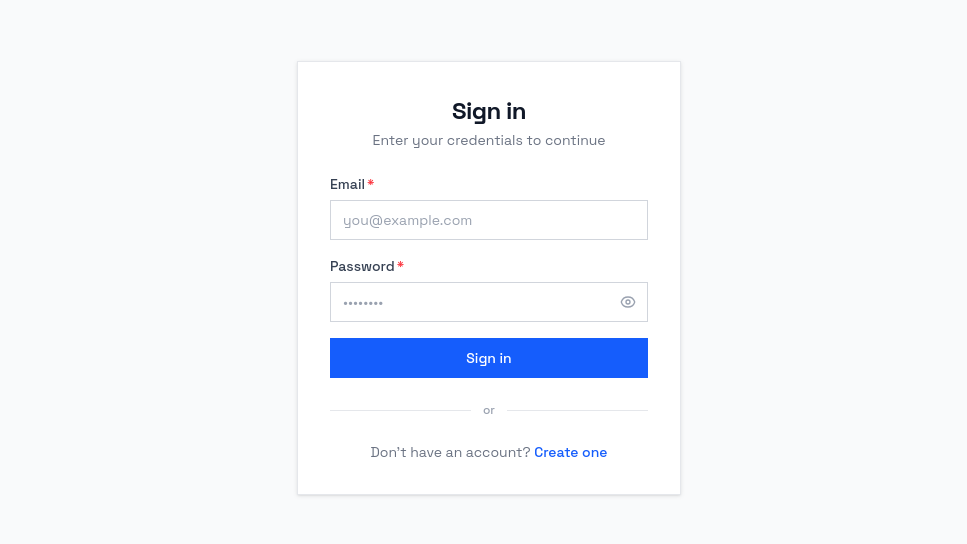
\includegraphics[width=\textwidth]{slike/manager-prijava.png}
\caption{Prijavna stran spletne aplikacije za vodje in kadrovsko službo.}
\label{fig:manager-prijava}
\end{figure}
\FloatBarrier

\section{Avtentikacija in nadzor dostopa}
\label{sec:sistem-avtentikacija}

Nova organizacija pridobi zaposlene prek povabil: kadrovska služba na naslov zaposlenega pošlje povabilo, ki ga zaledje shrani v tabelo \texttt{invitations} skupaj z zgoščeno vrednostjo enkratnega žetona. Zaposleni ob sprejemu povabila izbere geslo, zaledje pa ob prijavi preveri elektronski naslov z enkratno kodo (angl. One-Time Password, OTP), ki jo pošlje po elektronski pošti prek čakalne vrste, opisane v razdelku~\ref{sec:arhitektura}. Zaledje po petih zaporednih napačnih poskusih vnosa kode nadaljnje poskuse zavrne in zahteva ponoven začetek registracije, potekle ali že uporabljene kode pa zavrne takoj.

Ob uspešni prijavi zaledje izda dva žetona JWT: kratkoživ dostopni žeton, ki ga odjemalec hrani v pomnilniku in ga pošilja v glavi \texttt{Authorization}, ter dolgoživ osvežitveni žeton, ki ga zaledje shrani kot sejo (\texttt{sessions}) in odjemalcu vrne v piškotku, vezanem na napravo. Taka delitev omeji izpostavljenost dostopnega žetona, hkrati pa uporabniku ni treba gesla vnašati znova ob vsakem poteku dostopnega žetona. Ker si spletna aplikacija za vodje in administratorska aplikacija delita isto zaledno domeno, zaledje piškotka za navadne uporabnike in administratorja loči po imenu, dostopni žeton v glavi \texttt{Authorization} pa ima vedno prednost pred piškotkom, da preprečimo, da bi zastarel piškotek ene aplikacije preglasil žeton druge.

Vsak klic na zaščiteno pot gre skozi dve zaporedni varovali. Prvo (\texttt{JwtAuthGuard}) preveri veljavnost dostopnega žetona in iz njega prebere identiteto ter vlogo uporabnika. Poti, označene kot javne, preverjanje preskočijo. Drugo (\texttt{RolesGuard}) preveri, ali vloga uporabnika ustreza vlogam, ki jih zahteva klicana pot, sicer zahtevo zavrne s stanjem 403. Tabela~\ref{tab:vloge} povzame, katere vloge imajo dostop do posameznih sklopov funkcionalnosti.

\begin{table}[htbp]
\centering
\caption{Poenostavljen pregled dostopa do posameznih sklopov po vlogah.}
\label{tab:vloge}
\resizebox{\textwidth}{!}{%
\begin{tabular}{lccccc}
\toprule
Sklop & Admin & HR & Vodja & Zaposleni & Superadmin \\
\midrule
Lastni dogodki, izmene, odsotnosti & \checkmark & \checkmark & \checkmark & \checkmark & -- \\
Urejanje izmen tima & \checkmark & \checkmark & \checkmark & -- & -- \\
Nastavitve razporejanja & \checkmark & \checkmark & -- & -- & -- \\
Upravljanje zaposlenih in povabil & \checkmark & \checkmark & \checkmark & -- & -- \\
Potrjevanje odsotnosti in popravkov & \checkmark & \checkmark & \checkmark & -- & -- \\
Organizacije čez celotno platformo & -- & -- & -- & -- & \checkmark \\
\bottomrule
\end{tabular}%
}
\end{table}
\FloatBarrier

\section{Upravljanje zaposlenih}
\label{sec:sistem-zaposleni}

Kadrovska služba v spletni aplikaciji ustvari povabilo z elektronskim naslovom, imenom, priimkom in vlogo novega sodelavca. Zaledje ustvari zapis v tabeli \texttt{invitations} in po čakalni vrsti odloži pošiljanje elektronske pošte s povezavo do sprejema povabila. Ko zaposleni povabilo sprejme in izbere geslo, zaledje ustvari nov zapis v tabeli \texttt{users} z ustrezno vlogo in organizacijo ter pripadajoč \texttt{employee\_profiles} z osnovnimi kadrovskimi podatki, povabilo pa označi kot sprejeto. Kadrovska služba lahko kadar koli pregleduje seznam zaposlenih, ureja podatke posameznega profila (delovno mesto, oddelek, najvišje tedensko število ur) ali prekliče še nesprejeto povabilo.

\section{Evidenca delovnega časa}
\label{sec:sistem-cas}

Zaposleni v mobilni aplikaciji ob prihodu, odhodu, začetku ali koncu odmora ter podobnih dogodkih sproži enostaven klic, ki v tabelo \texttt{work\_events} doda vrstico s tipom dogodka in časovnim žigom. Ker se dogodki beležijo sproti in je napačen pritisk pogost, zaposleni namesto neposrednega urejanja že zabeleženega dogodka odda zahtevek za popravek: ta se shrani v tabelo \texttt{event\_change\_requests} skupaj z zahtevanim tipom dogodka, časom in razlogom, obstoječi dogodek pa ostane nespremenjen do odobritve. Vodja v spletni aplikaciji pregleduje čakajoče zahtevke svojega tima. Ob odobritvi zaledje glede na vrsto zahtevka (dodaj, uredi, izbriši) ustrezno spremeni izvorni zapis v \texttt{work\_events} in zahtevek označi kot odobren, ob zavrnitvi pa zgolj zabeleži razlog in izvorni dogodek pusti nespremenjen.

\section{Razporejanje izmen}
\label{sec:sistem-razporejanje}

Vodja urnik lahko sestavlja ročno, izmeno po izmeno, ali s ponavljajočimi se vzorci in predlogami zasedenosti, opisanimi v razdelku~\ref{sec:podatkovni-model}. Izmena brez dodeljenega zaposlenega je označena kot odprta, kateri koli ustrezen zaposleni jo lahko v mobilni ali spletni aplikaciji prevzame, zaledje pa ob tem preveri, da se izmena ne prekriva z že dodeljenimi izmenami tega zaposlenega. Slika~\ref{fig:manager-urnik} prikazuje tedenski pregled urnika v spletni aplikaciji za vodje.

\begin{figure}[htbp]
\centering
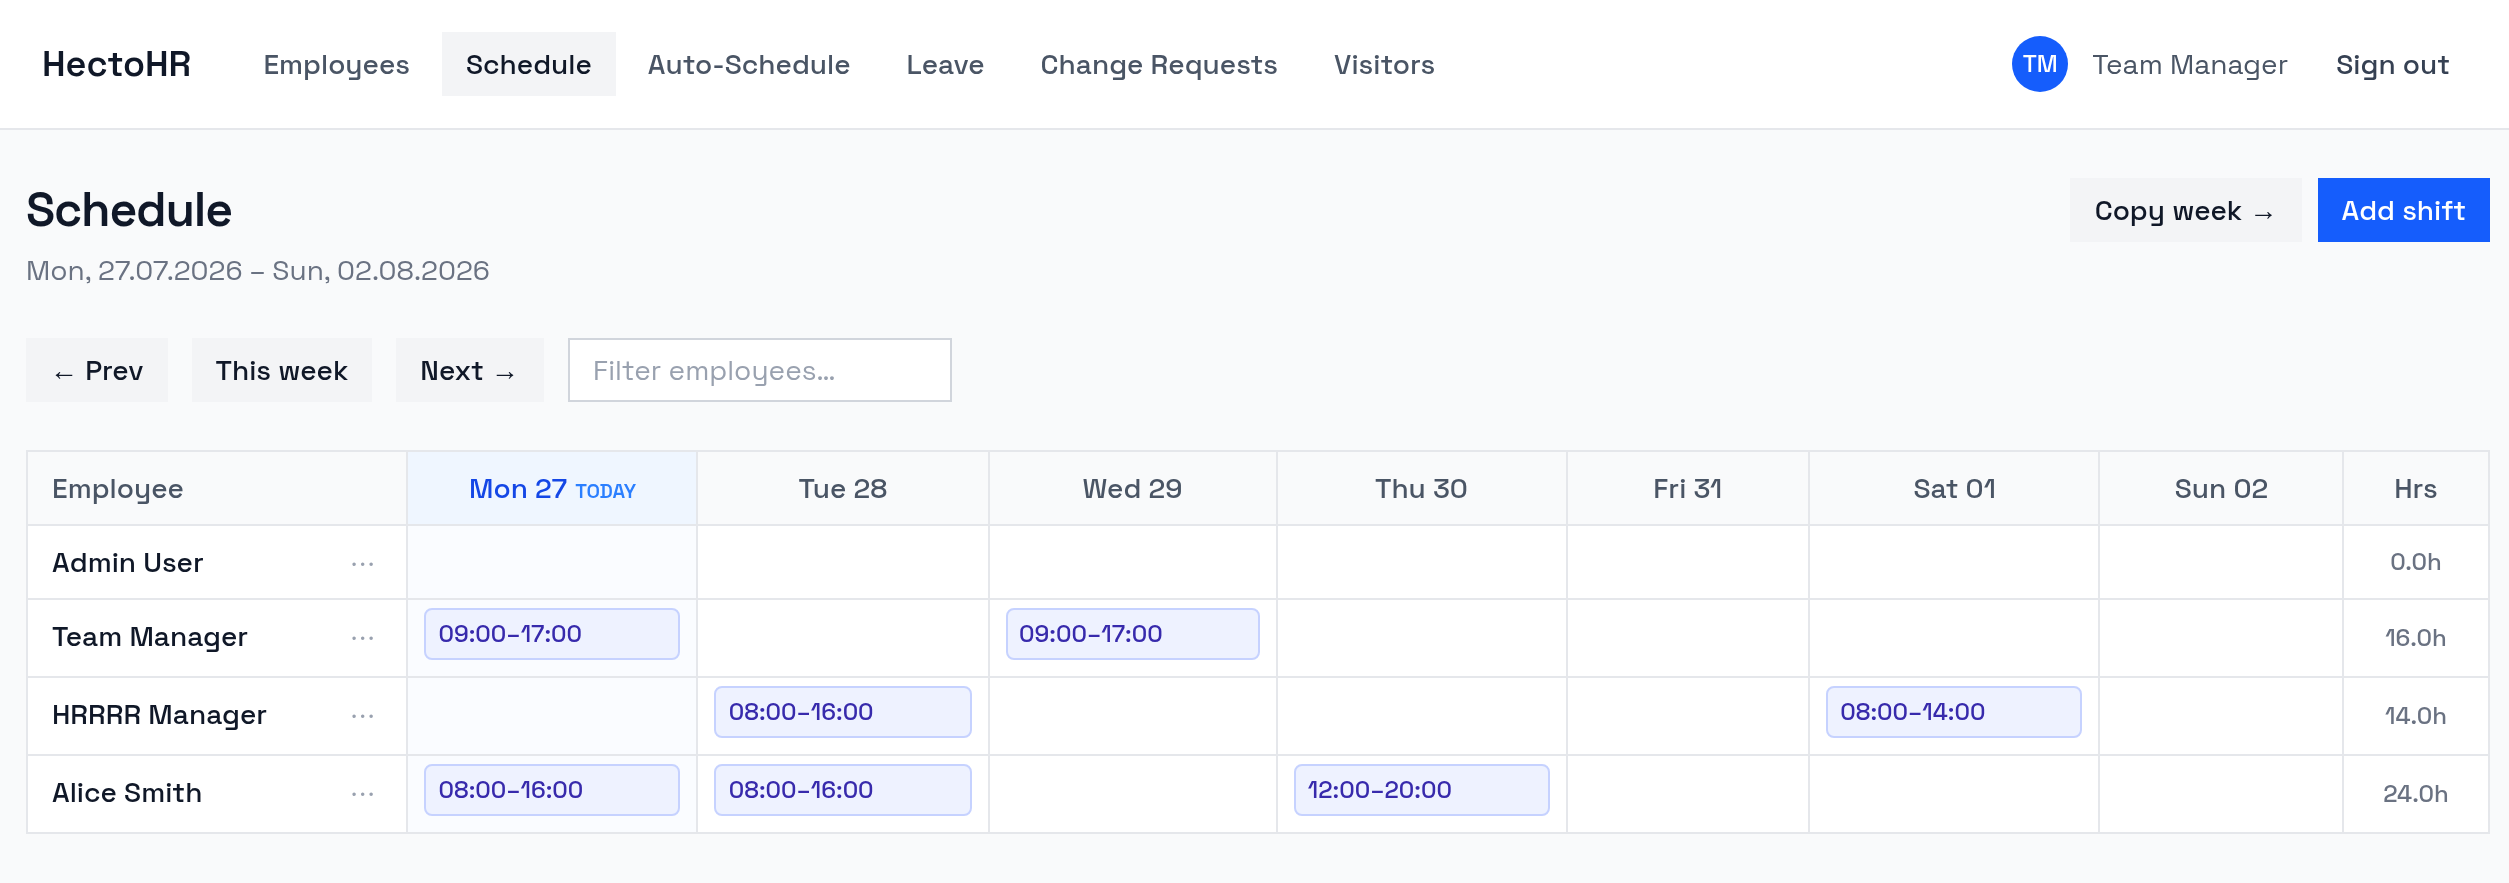
\includegraphics[width=\textwidth]{slike/manager-urnik.png}
\caption{Tedenski pregled urnika v spletni aplikaciji za vodje.}
\label{fig:manager-urnik}
\end{figure}
\FloatBarrier

Za samodejno sestavljanje urnika vodja izbere časovno obdobje, za katero želi predlog. Zaledje najprej iz predlog zasedenosti za to obdobje ustvari manjkajoče izmene, nato pa ustvari osnutek urnika (\texttt{schedule\_drafts}) in nad njim požene reševalnik. Reševalnik izmene obravnava kronološko in za vsako izmeno med kandidati izbere najprimernejšega zaposlenega, kot prikazuje algoritem~\ref{alg:solver}.

\begin{algorithm}[htbp]
\caption{Poenostavljen potek požrešnega reševalnika razporejanja}
\label{alg:solver}
\begin{algorithmic}[1]
\Function{RazporediOsnutek}{izmene, zaposleni, nastavitve}
    \State razvrsti \textit{izmene} kronološko po datumu in času začetka
    \State stanje $\gets$ prazna preslikava (zasedeni termini in tedenske ure na zaposlenega)
    \For{vsako izmeno $s$ v \textit{izmenah}}
        \State ocene $\gets$ []
        \For{vsakega zaposlenega $z$ v \textit{zaposlenih}}
            \State izračunaj primernost $z$ za $s$: odsotnosti, razpoložljivost, prekrivanje, tedenska omejitev ur, minimalni počitek
            \State ocene.dodaj(($z$, primeren?, preferenca, tedenske ure))
        \EndFor
        \State primerni $\gets$ filtriraj ocene po primeren?
        \If{primerni ni prazen}
            \State najboljši $\gets$ tisti z najvišjo preferenco (izbrana strategija razveže neodločeno po tedenskih urah)
            \State dodeli $s$ najboljšemu, posodobi njegovo stanje
        \Else
            \State označi $s$ kot nezasedeno, zabeleži razlog (npr.\ ni razpoložljivega zaposlenega)
        \EndIf
    \EndFor
    \State \Return predlagane dodelitve
\EndFunction
\end{algorithmic}
\end{algorithm}
\FloatBarrier

Organizacija lahko izbere eno izmed treh strategij razvrščanja, ki določajo, kateremu kriteriju reševalnik pri izbiri med primernimi zaposlenimi da prednost:

\begin{itemize}
    \item \texttt{preference\_first} -- reševalnik najprej izbere zaposlenega z najvišjo preferenco za dani termin, med enako preferenčnimi zaposlenimi pa tistega z manj že dodeljenimi urami v tednu.
    \item \texttt{fairness\_first} -- obrne vrstni red kriterijev: prednost dobi zaposleni z manj že dodeljenimi urami v tednu, preferenca pa odloči šele, če imata dva zaposlena enako število ur.
    \item \texttt{preference\_only} -- razvršča enako kot \texttt{preference\_first}, a med primerne za dani termin uvrsti le tiste zaposlene, ki so ga izrecno označili kot preferiranega, s čimer se preferenca upošteva strogo, ne le kot kriterij razvrščanja.
\end{itemize}

Ker gre za požrešno hevristiko in ne za eksaktni reševalnik, kot smo utemeljili v razdelku~\ref{sec:razporejanje-osebja}, dobljeni osnutek ni nujno optimalen: vodja ga v spletni aplikaciji lahko pregleda, posamezne dodelitve ročno spremeni in šele nato objavi. Slika~\ref{fig:manager-samodejno-razporejanje} prikazuje osnutek urnika za en teden, kjer je reševalnik vseh deset izmen uspešno dodelil štirim zaposlenim, vsako izmeno enemu izmed njih. Med objavo zaledje vsem zaposlenim z dodeljeno izmeno po čakalni vrsti pošlje potisno obvestilo, če pa to ni mogoče, obvestilo pošlje po elektronski pošti.

\begin{figure}[htbp]
\centering
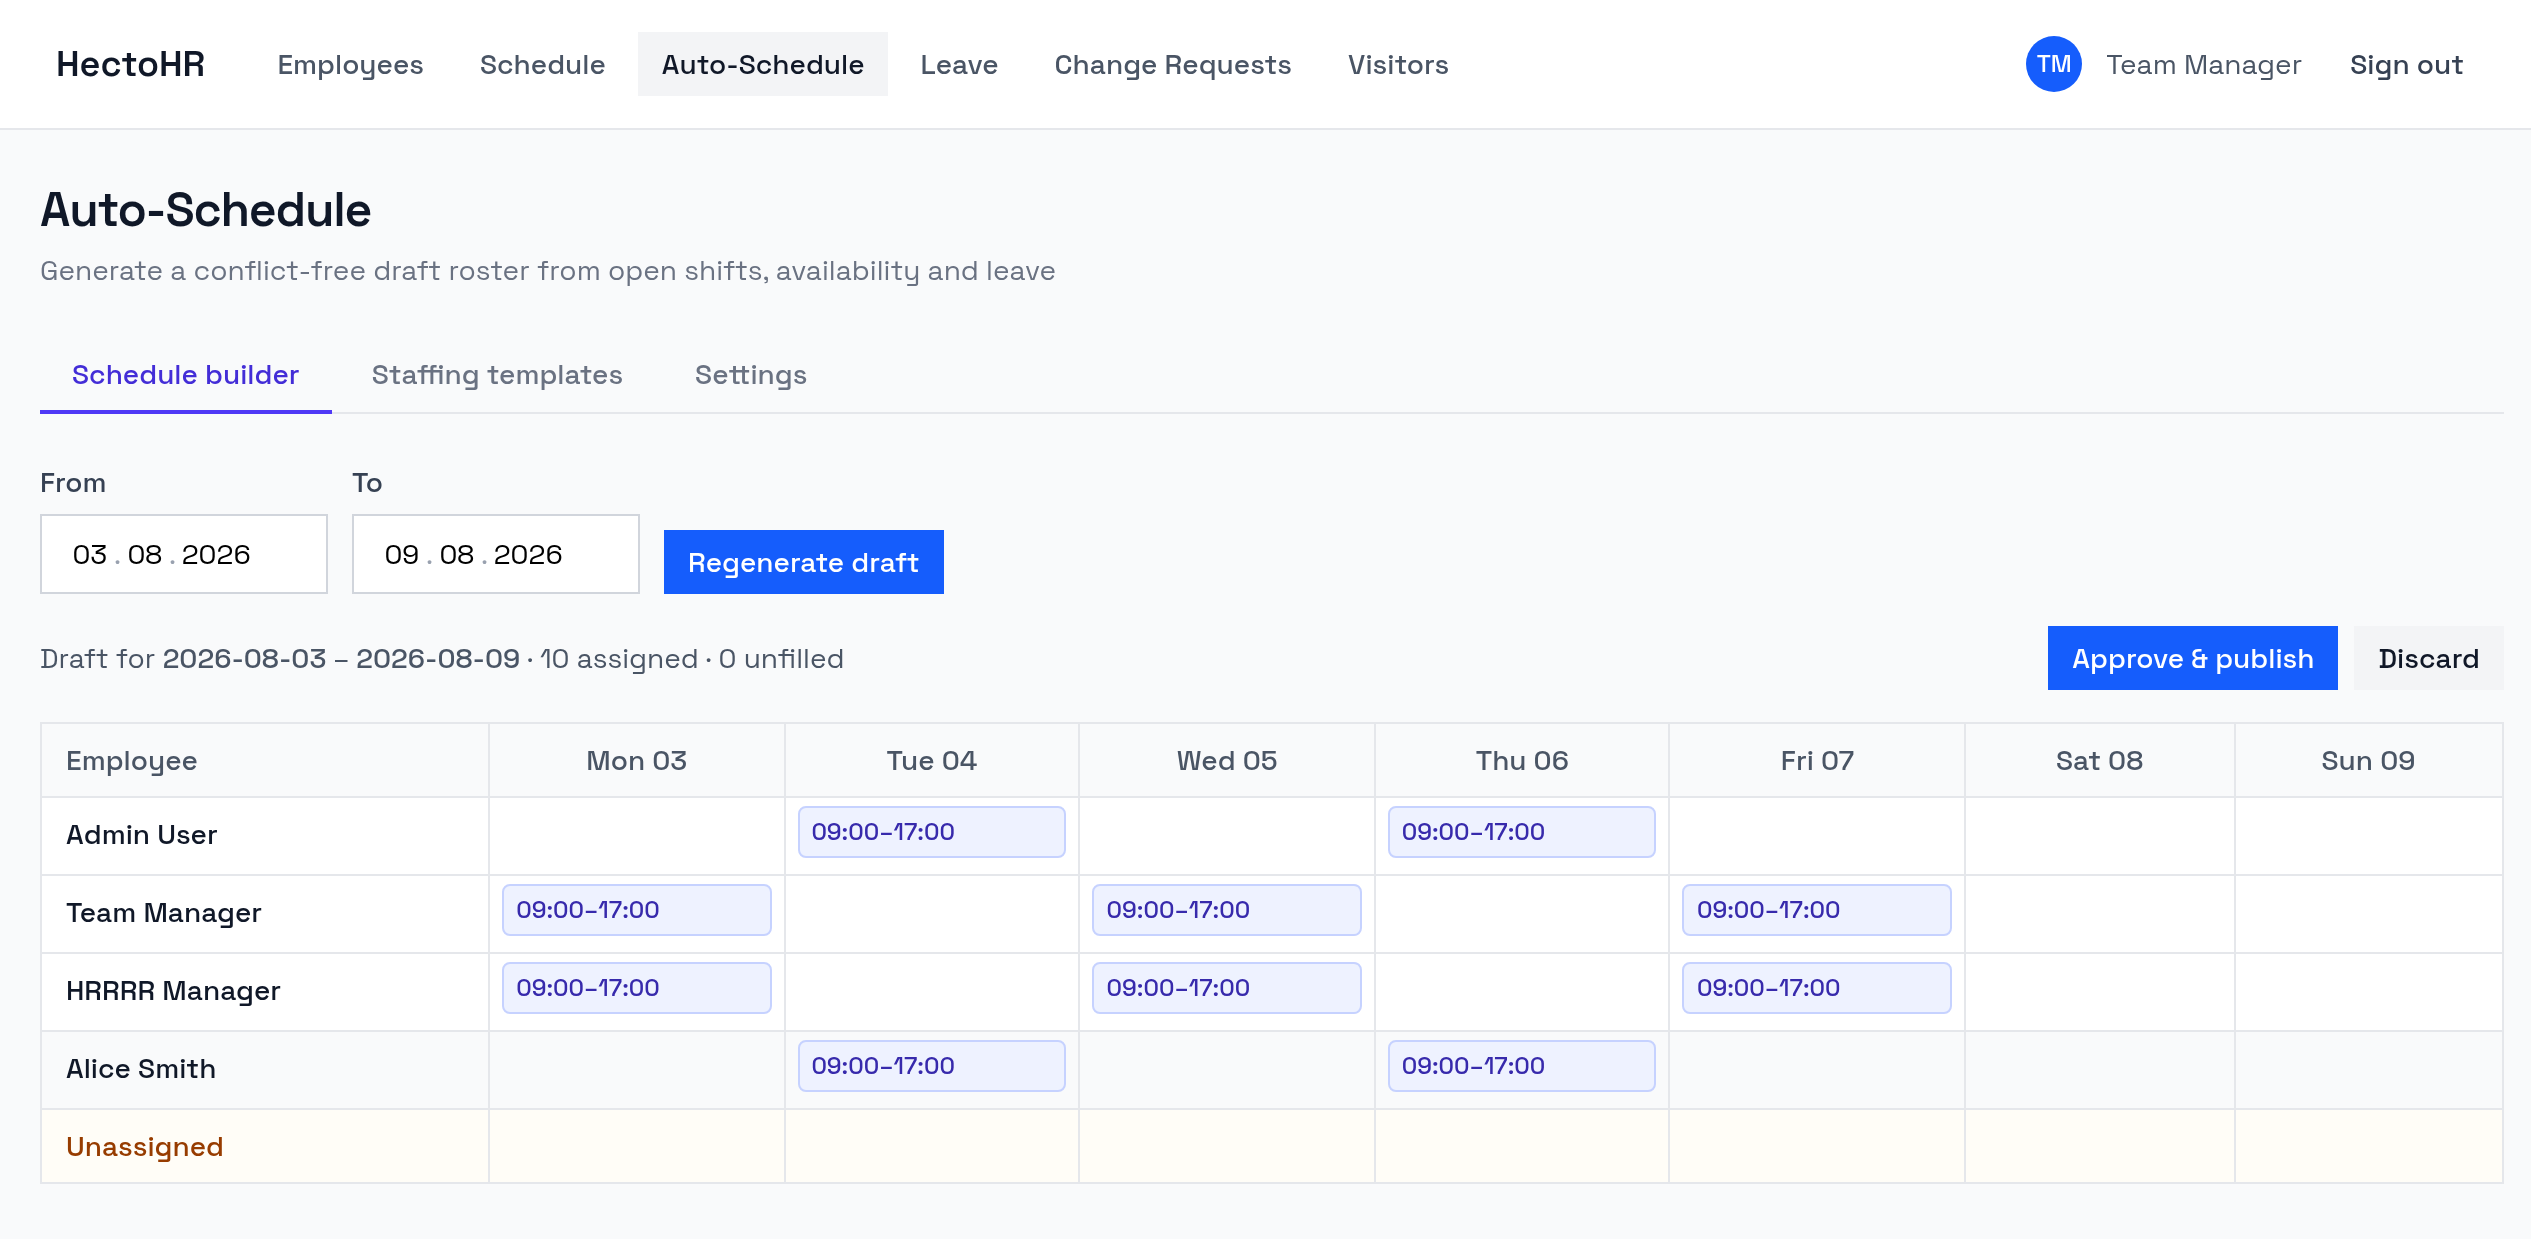
\includegraphics[width=\textwidth]{slike/manager-samodejno-razporejanje.png}
\caption{Osnutek urnika, ki ga je predlagal reševalnik za samodejno razporejanje.}
\label{fig:manager-samodejno-razporejanje}
\end{figure}
\FloatBarrier

\section{Upravljanje odsotnosti}
\label{sec:sistem-odsotnosti}

Kadrovska služba za organizacijo nastavi tipe odsotnosti (na primer letni dopust, bolniška odsotnost) z lastnostmi, ali je tip plačan in koliko dni na leto pripada posameznemu zaposlenemu privzeto. Zaledje nato za vsakega zaposlenega in leto ustvari ustrezen zapis stanja odsotnosti (\texttt{leave\_balances}). Zaposleni v mobilni aplikaciji odda zahtevek za odsotnost z izbranim tipom in obdobjem, zaledje pa samodejno izračuna število delovnih dni in stanje označi kot čakajoče. Vodja ali kadrovska služba zahtevek odobri ali zavrne. Ob odobritvi zaledje čakajoče dni prenese med izrabljene, ob zavrnitvi pa jih vrne nazaj v razpoložljivo stanje. Kadrovska služba lahko dneve v stanju odsotnosti tudi ročno popravi, na primer ob prenosu neizrabljenih dni iz preteklega leta. Slika~\ref{fig:manager-odsotnosti} prikazuje pregled čakajočih zahtevkov za odsotnost v spletni aplikaciji za vodje, skupaj z gumboma za odobritev in zavrnitev.

\begin{figure}[htbp]
\centering
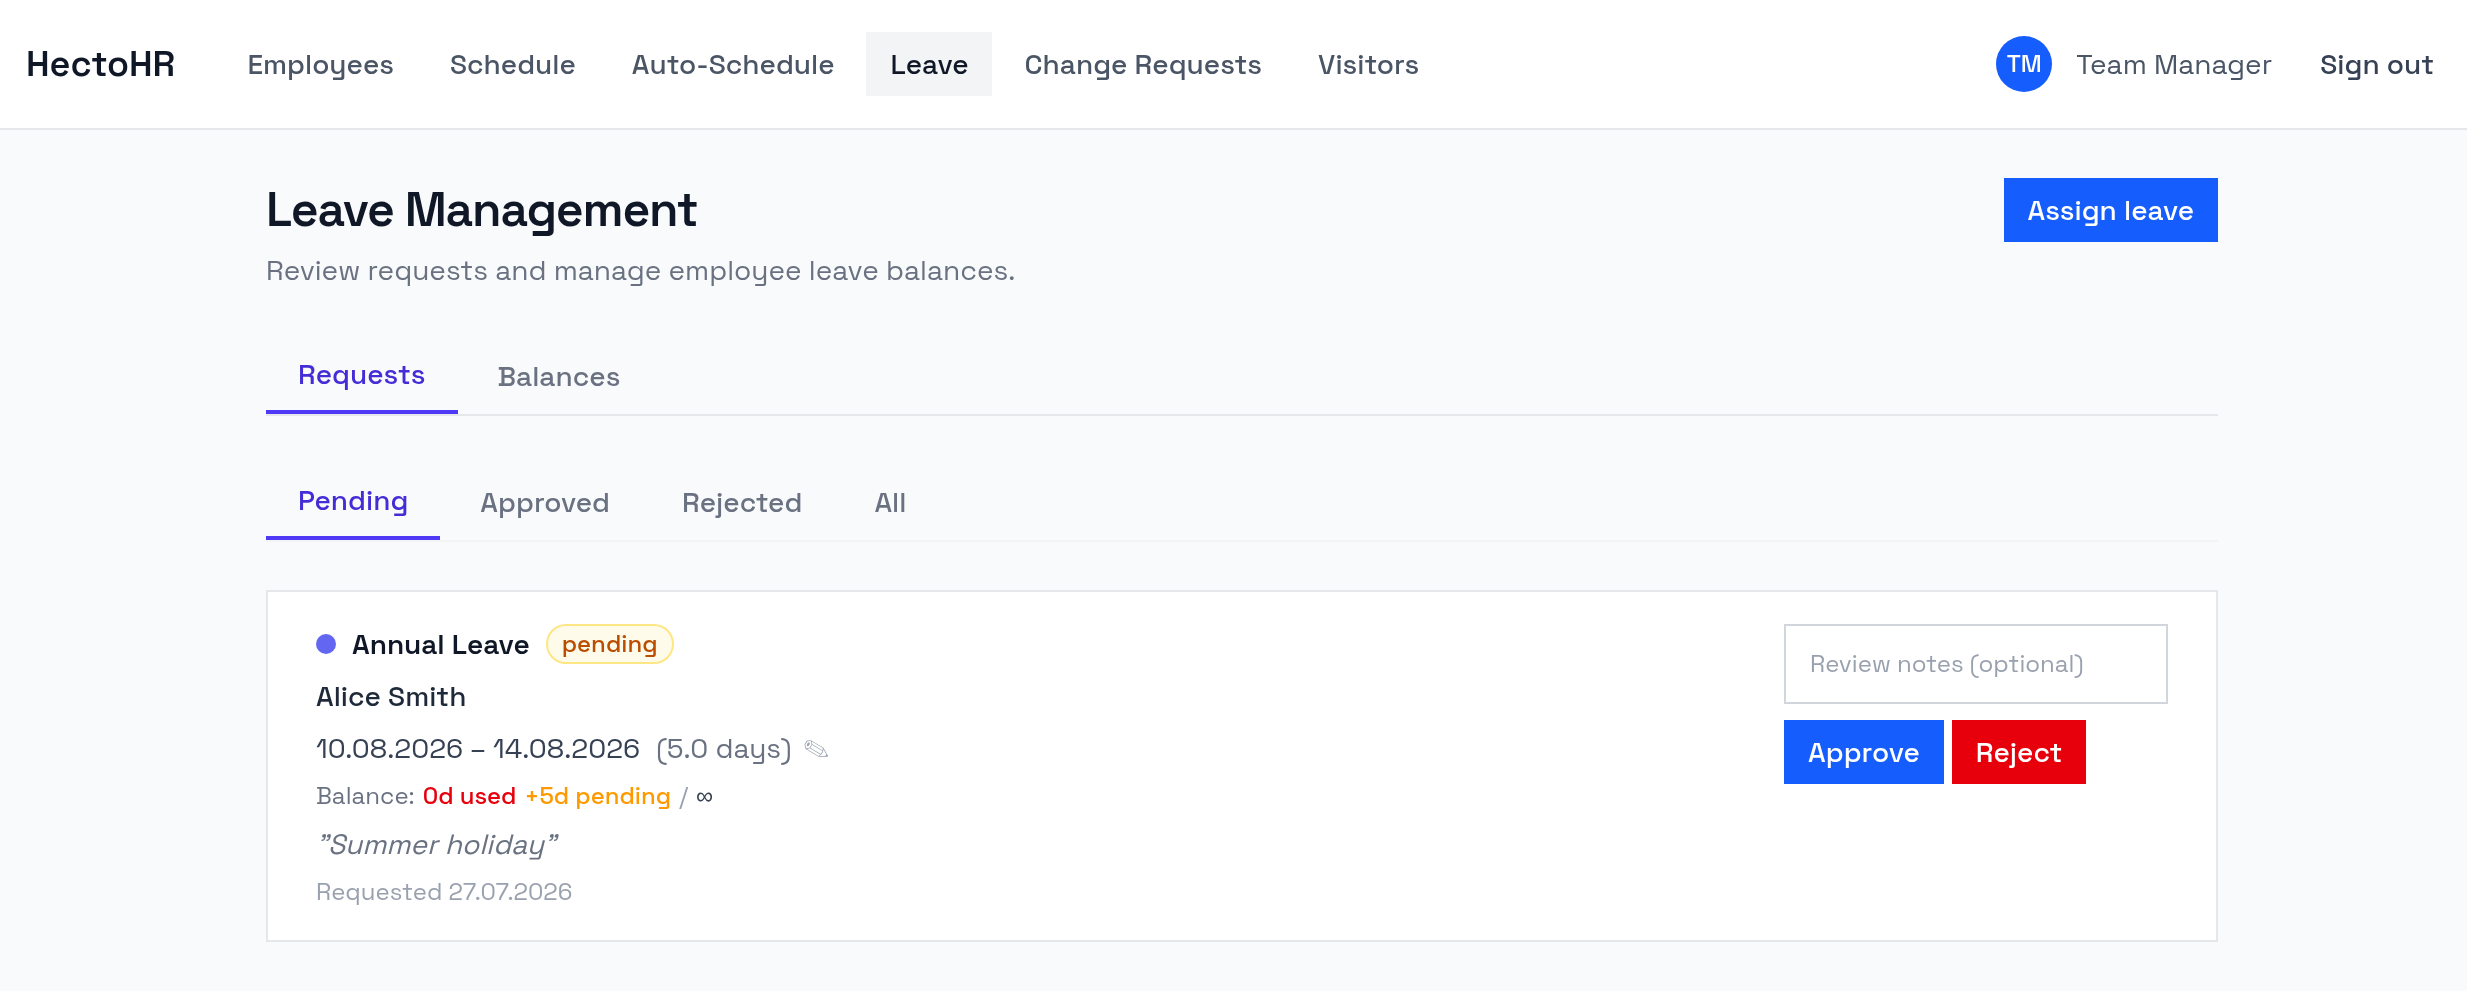
\includegraphics[width=\textwidth]{slike/manager-dopusti.png}
\caption{Pregled čakajočih zahtevkov za odsotnost.}
\label{fig:manager-odsotnosti}
\end{figure}
\FloatBarrier

\section{Evidenca obiskov}
\label{sec:sistem-obiski}

Poleg osrednjih kadrovskih procesov sistem vključuje še dodaten, samostojen modul za evidenco obiskov na recepciji organizacije, ki smo ga omenili že v uvodu (razdelek~\ref{sec:cilji}). Modul teče kot mobilna aplikacija na poljubni napravi na recepciji, najpogosteje tablici, ki jo je treba pred uporabo z zaledjem enkratno seznaniti (parjenje), s čimer vzpostavi lastno zaupanje do zaledja, neodvisno od uporabniške prijave.

Administrator organizacije v spletni aplikaciji ustvari paritveno kodo z omejeno veljavnostjo in imenom naprave (na primer ``Recepcija''), to kodo pa nato enkratno vnese v kiosk aplikacijo na tablici. Zaledje ob uspešnem parjenju kodo porabi in tablici izda dolgoživ žeton naprave, ki ga kiosk aplikacija odslej pošilja namesto uporabniškega žetona JWT. Poti \texttt{/kiosk/*} so zato v celoti izvzete iz varoval, opisanih v razdelku~\ref{sec:sistem-avtentikacija}, in namesto tega preverjajo izključno veljavnost žetona naprave. S tem se izognemo temu, da bi moral vsak obiskovalec za enkraten obisk imeti svoj uporabniški račun.

Obiskovalec na tablici vnese ime in namen obiska ter se podpiše na zaslon, kiosk aplikacija podpis kot sliko naloži neposredno v objektno shrambo, opisano v razdelku~\ref{sec:arhitektura}, zaledje pa ustvari zapis obiska (tabela \texttt{visits}) s časom prihoda in sklicem na naloženo sliko. Recepcija obiskovalca ob odhodu na tablici označi kot odjavljenega, če pa to pozabi, zaledje obisk samodejno zapre ob koncu dne. Zaposleni z ustrezno vlogo lahko v spletni aplikaciji kadar koli preverijo, kdo je trenutno v prostorih organizacije, in pregledajo pretekle obiske.

\section{Administracija platforme}
\label{sec:sistem-admin}

Administrator platforme (vloga \texttt{superadmin}) do sistema dostopa prek ločenega prijavnega mesta, ki sprejme le uporabnike s to vlogo. Ta uporabnik ne pripada nobeni organizaciji in ni ustvarjen prek običajnega vabila, temveč izključno prek namenskega ukaza ob namestitvi sistema. Administratorska aplikacija administratorju omogoča iskanje in pregled organizacij, kar prikazuje slika~\ref{fig:admin-organizacije}, ter uporabnikov čez celotno platformo, onemogočanje ali izbris organizacije, ki posledično prijavo uporabnikom te organizacije zavrne, ter prisilno odjavo ali ponastavitev gesla posameznega uporabnika. Vsako spremembo, ki jo administrator izvede, zaledje zabeleži v tabelo \texttt{admin\_audit\_logs} skupaj s stanjem zapisa pred spremembo in po njej, kar omogoča poznejšo sledljivost posegov, zahtevano v razdelku~\ref{sec:zahteve}.

\begin{figure}[htbp]
\centering
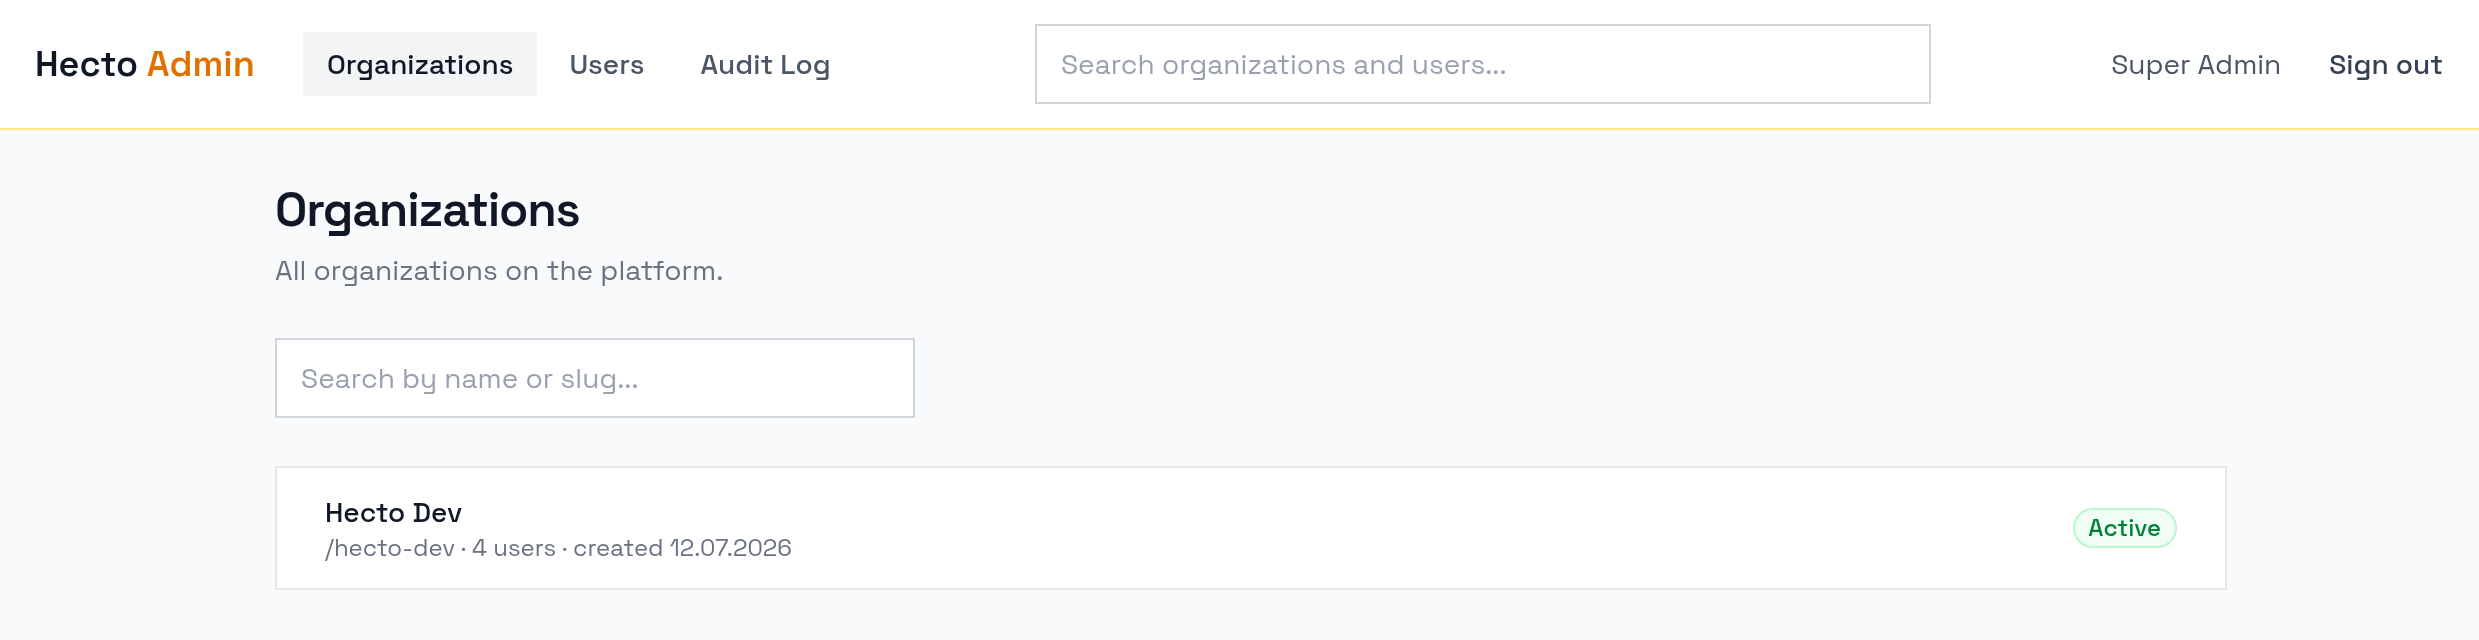
\includegraphics[width=\textwidth]{slike/admin-organizacije.png}
\caption{Pregled organizacij v administratorski aplikaciji.}
\label{fig:admin-organizacije}
\end{figure}
\FloatBarrier

\chapter{Evalvacija}
\label{ch:evalvacija}

V tem poglavju preverimo hipotezi H2 in H3 iz razdelka~\ref{sec:hipoteze} tako, da razvito rešitev preizkusimo s testnimi uporabniki in njihovo oceno zaznane uporabnosti ovrednotimo s standardiziranim vprašalnikom System Usability Scale (SUS)~\cite{brooke1996sus}, ki smo ga izbrali med sorodnimi vprašalniki.

\section{Udeleženci in postopek}
\label{sec:eval-postopek}

Za testiranje smo povabili 12 testnih uporabnikov izmed kolegov, družinskih članov in prijateljev, katerih demografsko in poklicno ozadje ustreza ciljni skupini aplikacije (zaposleni v manjših podjetjih, vodje manjših timov). Povprečna starost udeležencev je znašala 27,0 let (standardni odklon 9,7 leta), med njimi so bile 3 ženske in 9 moških. Vsak udeleženec je v vlogi zaposlenega, vodje ali kadrovske službe opravil kratek nabor nalog, ki pokrivajo osrednje module sistema, opisane v poglavju~\ref{ch:sistem}:

\begin{enumerate}
    \item prijava v sistem in beleženje dogodka delovnega časa (prihod, odmor, odhod) v mobilni aplikaciji,
    \item oddaja zahtevka za dopust in, v vlogi vodje ali kadrovske službe, odobritev zahtevka drugega udeleženca,
    \item v vlogi vodje: samodejno generiranje osnutka urnika za teden dni, pregled predlaganih dodelitev in objava urnika,
    \item prevzem odprte izmene v vlogi zaposlenega.
\end{enumerate}

Po zaključenih nalogah je vsak udeleženec izpolnil vprašalnik SUS, predstavljen v razdelku~\ref{sec:eval-sus}. Testiranje je potekalo samostojno na lastni napravi, izvedba naštetih nalog (brez izpolnjevanja vprašalnika) pa je v povprečju trajala 10 minut.

\section{Vprašalnik SUS}
\label{sec:eval-sus}

Vprašalnik SUS sestavlja deset trditev, na katere udeleženec odgovori s petstopenjsko lestvico strinjanja, pri čemer 1 pomeni ``sploh se ne strinjam'' in 5 ``popolnoma se strinjam''. Trditve smo prevedli v slovenščino:

\begin{enumerate}
    \item Mislim, da bi to aplikacijo rad(-a) uporabljal(-a) pogosto.
    \item Aplikacija se mi je zdela po nepotrebnem zapletena.
    \item Zdelo se mi je, da je aplikacijo enostavno uporabljati.
    \item Mislim, da bi za uporabo te aplikacije potreboval(-a) pomoč tehnične osebe.
    \item Zdelo se mi je, da so različne funkcije aplikacije dobro povezane med seboj.
    \item Zdelo se mi je, da je v aplikaciji preveč neskladnosti.
    \item Domnevam, da bi se večina ljudi zelo hitro naučila uporabljati to aplikacijo.
    \item Aplikacija se mi je zdela zelo okorna za uporabo.
    \item Pri uporabi aplikacije sem se počutil(-a) samozavestno.
    \item Preden sem lahko začel(-a) uporabljati aplikacijo, sem se moral(-a) naučiti veliko stvari.
\end{enumerate}

Trditve z lihimi zaporednimi številkami so pozitivno naravnane (višja ocena pomeni boljši rezultat), s sodimi pa negativno (višja ocena pomeni slabši rezultat). Posamezno oceno SUS izračunamo tako, da pri lihih trditvah od odgovora odštejemo 1, pri sodih pa odgovor odštejemo od 5, dobljene vrednosti seštejemo in zmnožimo z 2,5, kar da končno oceno na lestvici od 0 do 100. Bangor in sodelavci~\cite{bangor2009determining} so oceni SUS dodali pridevniško lestvico, katere mejne vrednosti je potrdil tudi Hertzum~\cite{hertzum2026meta}: povprečna ocena 85 ustreza pridevniku ``odlično'', 71 ``dobro'', 51 pa ``ok'', torej približno povprečju. Za razvrščanje rezultatov v nadaljevanju te meje poenostavimo takole: oceno nad 85 uvrščamo med ``odlično'', med 71 in 85 med ``dobro'', okoli 51 predstavlja povprečje, pod 51 pa velja za slabo.

\clearpage
\section{Rezultati}
\label{sec:eval-rezultati}

Tabela~\ref{tab:sus-rezultati} povzame oceno SUS za vsakega izmed 12 udeležencev.

\begin{table}[htbp]
\centering
\caption{Individualne in povprečna ocena SUS.}
\label{tab:sus-rezultati}
\begin{tabular}{lc}
\toprule
Udeleženec & Ocena SUS \\
\midrule
U1  & 90,0 \\
U2  & 92,5 \\
U3  & 100,0 \\
U4  & 82,5 \\
U5  & 92,5 \\
U6  & 97,5 \\
U7  & 85,0 \\
U8  & 90,0 \\
U9  & 67,5 \\
U10 & 97,5 \\
U11 & 70,0 \\
U12 & 92,5 \\
\midrule
Povprečje & 88,1 \\
\bottomrule
\end{tabular}
\end{table}
\FloatBarrier

Povprečna ocena SUS znaša 88,1, kar po pridevniški lestvici sodi v razred ``odlično''. Devet od dvanajstih udeležencev doseže oziroma preseže mejo 85 (``odlično''), en udeleženec, z oceno 82,5, pade v razred ``dobro'', preostala dva pa v razred okoli povprečja (51), nobena ocena pa ne pade pod mejo povprečja ali v razred ``slabo''. Take rezultate lahko pripišemo predvsem preprostosti nabora testnih nalog.

Glede na dobljene rezultate hipotezo H3, da bodo uporabniki zaznano uporabnost aplikacije ocenili kot dobro, kar se bo pokazalo v povprečnem rezultatu SUS nad 71 točk, potrdimo. K hipotezi H2 o časovnem prihranku pri samodejnem razporejanju ne moremo podati enakovredno trdne trditve: v končni obliki vprašalnika ločenega vprašanja o prihranku časa v primerjavi z ročnim razporejanjem nismo vključili, zato nimamo neposredne kvantitativne potrditve. Posredno jo podpira podatek, da so udeleženci nalogo generiranja, pregleda in objave osnutka urnika med testiranjem opravili hitro in brez večjih zapletov, kar je skladno tudi z visoko oceno trditve o povezanosti funkcij aplikacije (trditev 5). Hipotezo H2 zato lahko na podlagi izvedene evalvacije potrdimo le delno. Za trdnejšo potrditev bi bilo treba, kot navajamo v razdelku~\ref{ch:zakljucek}, prihranek časa izmeriti neposredno.

\chapter{Zaključek}
\label{ch:zakljucek}

V diplomskem delu smo zasnovali in razvili spletno in mobilno aplikacijo za upravljanje delovnega časa in kadrovskih procesov, ki v enotnem sistemu združuje evidenco delovnega časa, razporejanje izmen z možnostjo samodejnega generiranja osnutka urnika in upravljanje odsotnosti, ob tem pa podpira dostop na osnovi vlog za administratorja, kadrovsko službo, vodjo in zaposlenega ter nadzorni vmesnik za upravljanje več organizacij na eni platformi. Dosegli smo vse cilje, opredeljene v razdelku~\ref{sec:cilji}: zajeli smo zahteve po vlogah, zasnovali podatkovni model in arhitekturo (poglavje~\ref{ch:nacrtovanje}), razvito rešitev opisali po modulih (poglavje~\ref{ch:sistem}) in jo ovrednotili s testnimi uporabniki (poglavje~\ref{ch:evalvacija}).

Glede na rezultate evalvacije hipotezo H3, da bodo uporabniki aplikacijo ocenili kot uporabno in enostavno za uporabo, potrdimo: povprečna ocena SUS na vzorcu 12 testnih uporabnikov je znašala 88,1, kar po pridevniški lestvici Bangorja in sodelavcev~\cite{bangor2009determining} sodi v razred ``odlično''. Hipotezo H2 o časovnem prihranku pri samodejnem razporejanju lahko na podlagi izvedene evalvacije potrdimo le delno, saj časovnega prihranka v primerjavi z ročnim razporejanjem nismo izmerili neposredno, temveč jo posredno podpira hitra in nemotena izvedba naloge razporejanja med testiranjem. Hipotezo H1, da enoten sistem zmanjša potrebo po ročnem usklajevanju podatkov med ločenimi orodji, neposredno nismo merili s testnimi uporabniki, temveč jo utemeljujemo z zasnovo samega sistema (poglavje~\ref{ch:nacrtovanje}), v katerem so evidenca delovnega časa, razporejanje izmen in odsotnosti od začetka povezani na skupnem podatkovnem modelu, ne da bi bilo med njimi potrebno ročno prenašanje podatkov. K podobnemu sklepu vodijo tudi raziskave s področja digitalizacije kadrovskih procesov: Mahmoud in sodelavci~\cite{mahmoud2025digitalhrm} na vzorcu zaposlenih pokažejo, da digitalni kadrovski informacijski sistemi statistično značilno zmanjšajo zapletenost nalog in potrebo po ročnem delu ter s tem izboljšajo učinkovitost kadrovske funkcije.

\section{Omejitve rešitve}

Razvita rešitev ima kljub doseženim ciljem več omejitev. Reševalnik za samodejno razporejanje je požrešna hevristika, ki izmene dodeljuje kronološko in ne poišče nujno globalno najboljše razporeditve za celotno obdobje, kot smo pojasnili v razdelkih~\ref{sec:razporejanje-osebja} in~\ref{sec:sistem-razporejanje}. Pri zahtevnejših urnikih z veliko omejitvami bi eksaktni ali metahevristični pristop lahko dal boljši rezultat, a na račun daljšega časa izvajanja in zahtevnejšega vzdrževanja kode. Evalvacija je potekala na majhnem, priložnostnem vzorcu udeležencev (kolegi, družina, prijatelji), zato dobljenih ocen SUS ne moremo posplošiti na širšo populacijo uporabnikov kadrovskih sistemov, vendar pa je potrebno povedati, da so udeleženci sodili v ciljno skupino uporabnikov. Sistem prav tako še ne podpira obračuna plač niti integracije z zunanjimi kadrovskimi ali računovodskimi sistemi, ki jih ponujajo nekatere komercialne rešitve iz razdelka~\ref{sec:komercialne-resitve}.

\section{Nadaljnje delo}

Rešitev bi lahko nadgradili v več smereh. Reševalnik razporejanja bi lahko razširili z možnostjo, da zaposleni za posamezno izmeno oddajo eksplicitno ponudbo namesto zgolj splošne preference, kar bi vodji dalo močnejši signal pri odločanju, ali pa reševalnik nadomestili z metahevrističnim oziroma eksaktnim pristopom, na primer s celoštevilskim programiranjem, ki bi lahko poleg zasedenosti optimiziral tudi strošek dela. Smiselna razširitev bi bila tudi podpora obračunu plač na podlagi evidentiranega delovnega časa. Evalvacijo bi bilo koristno ponoviti na večjem in bolj raznolikem vzorcu uporabnikov, morda v obliki daljšega uporabniškega preizkusa v realnem podjetju, kar bi omogočilo tudi merjenje dejanskega prihranka časa pri razporejanju izmen, ne le subjektivne ocene uporabnikov.


%%%%%%%%%%%%%%%%%%%%%%%%%%%%%%%%%%%%%%%%
% LITERATURA
%%%%%%%%%%%%%%%%%%%%%%%%%%%%%%%%%%%%%%%%

\printbibliography[heading=bibintoc]

\end{document}
